\picturechapter{Modular antibody \emph{de novo} sequence analysis using multi-tier LC-MS/MS data}{Chaptercovers/ch5.pdf} \label{ch-5}
\vspace*{0.25cm}

{\footnotesize Sebastiaan C. de Graaf, Douwe Schulte, A. Bondt, Max Hoek, Weiwei Peng, Sem Tamara, Joost Snijder, Richard A. Scheltema, Albert J.R. Heck}
%%
\begin{center}
  \vspace{3cm}
  \includegraphics[]{Chapter.5/Figures/Ch5.png}
  \vspace{0.25cm}
\end{center}

\begin{flushleft}
  \vspace*{\fill}
  \rule{\textwidth}{1pt}\\[0cm]
\end{flushleft}

\begin{abstract102}
  Antibodies form an important class of biomolecules that are produced by the immune system to defend us against infections. Their importance is underlined by their successful use as therapeutic agents, enabled by their production as recombinant monoclonal proteins (mAbs). Prior to development of an antibody lead, identification of the amino acid sequence needs to be achieved. Commonly B-cell sequencing is used to identify the DNA/RNA sequences that lead to the antibodies of interest, although only a small subset of the B cells produce antibodies that end up in circulation. More recently mass spectrometry-based (MS) methods have been used for sequencing, with the added benefit that this is a direct approach to extract the sequence of the protein in circulation, thereby potentially providing insights into post-translational modifications. Both approaches have their implicit challenges, and the complete extraction of the amino acid sequence is still difficult to achieve. In MS-based approaches mostly shotgun proteomics has been applied, where the antibody is digested into peptides prior to identification. With such an approach, gaps in sequence coverage often arise, mostly in the complementarity-determining regions (CDRs) of the antibody that are responsible for the recognition and binding of infectious agents. Here, we demonstrate that by combining shotgun proteomics with middle-down (MD) proteomics, where the protein or large fragments thereof are measured intact, these gaps can be filled and better information on the sequence can be extracted. We therefore developed and described here software solutions to iteratively integrate data from BU and MD proteomics.
\end{abstract102}
\thumbforchapter

\section{Introduction}
\lettrine[lraise=0.1, nindent=0em, slope=-.5em]{A}{ntibodies}, or immunoglobulins, are one of the cornerstones of the human immune system and are abundantly present in various bodily fluids, such as serum, saliva, milk, the lumen of the gut, and cerebrospinal fluid \cite{schroeder2010structure}. Because of their important role in combatting infectious diseases, immunoglobulins have been intensively studied and in the last decades have taken centre stage for the development of novel therapeutics \cite{kaplon2021antibodies, marks2020how, raybould2020thera-sabdab:}. In the last decade, antibodies have become the best-selling drugs in the market, notably in 2018 eight of the top ten bestselling drugs were biologics.
New antibody leads for biotherapeutics can be extracted from various sources, such as immunized animals or recovered patients who carry pathogen neutralizing antibodies \cite{bornholdt2016isolation, corti2016protective, valgardsdottir2021identification}. The incredible potential for diversity of immunoglobulin molecules in the human body, with over 10\textsuperscript{15} theoretically possible sequences \cite{schroederjr.2006similarity, briney2019commonality}, indicates that each antigen exposure may lead to a unique, personalized (polyclonal) antibody response. One way to chart the antibody repertoire is to sequence the B-cell receptors of all B cells that can produce antibodies. It is however thought that only a marginal fraction of all these B cells indeed produce immunoglobulin proteins that end up in circulation, making this an inefficient undertaking. Alternatively and more ideal, investigation and sequencing of antibodies occurs directly at the protein level \cite{hom2022exploring}.
Mass spectrometry (MS) has become the method of choice for analysing protein mixtures \cite{altelaar2013next-generation, aebersold2016mass-spectrometric}, but sequencing polyclonal antibody mixtures still poses one of the major remaining challenges \cite{sen2017automated, peng2021mass, srzentić2020interlaboratory}. Most protein analyses by MS are performed by peptide-centric proteomics, also called shotgun or bottom-up (BU) proteomics, where the presence and relative abundance of proteins is inferred from peptides obtained by digesting the proteins with proteases, prior to sequencing. For the identification, this approach makes use of a protein sequence database to generate theoretical peptides from which the expected precursor mass and fragmentation spectrum is generated \cite{aebersold2003mass}. A sequence database is however not available for the full repertoire of antibodies, as their sequences are the result of the recombination and mutation of several genes encoded by many different alleles in each person. An option to sequence antibodies by shotgun proteomics is by using \emph{de novo} sequence analysis, where peptide sequences are directly determined from the fragmentation spectra. The resulting short peptide \emph{reads}, typically 5-25 amino acid residues in length, are assembled into longer \emph{contigs} or even full-length \emph{protein chain} sequences \cite{sen2017automated, tran2016complete, guthals2012shotgun}. A factor that makes read assembly for antibodies particularly difficult is that the sequence of both the light- and heavy chain of an antibody are made up of alternatingly conserved and hypervariable sequence domains \cite{charlesajaneway2001generation, alberts2002generation}. Fortunately, the quality of software platforms for \emph{de novo} sequence analysis of antibodies by MS is steadily increasing \cite{graaf2022perspective}. Virtually all published platforms make use of homologous sequence templates \cite{sen2017automated, tran2016complete, schulte2022template-based, castellana2010template}, obtained by comparing experimental data to an immunogenetic database such as the IMGT \cite{lefranc2003imgt, lefranc2020immunoglobulins}. The commercially available antibody sequencing platform Supernovo for example takes BU data as an input and returns a full-length sequence, along with the determined germline template sequences \cite{sen2017automated}. Through recent development in software and mass spectrometry results of these approaches may now lead to correct sequencing, albeit only for monoclonal antibody samples \cite{peng2021mass}. However, established software solutions in the field, including Supernovo, cannot yet sequence antibodies in polyclonal mixtures with equal success.
Recent advances in instrumentation, separation, sample preparation and computational power have facilitated protein-centric proteomics (also called top-down proteomics). This enables the simultaneous analysis of an entire protein, removing the need for protein inference \cite{toby2016progress}. This approach is very enticing as it side-steps the need for assembling peptide sequences into a full protein sequence. While the field has not yet matured to yield spectra that can routinely be used for confident \emph{de novo} sequencing without additional data, the continuous advances indicate that the future of antibody sequence analysis will surely include these techniques as a complementary source of information to the more established peptide-centric (BU) analyses. One particularly striking example of this is the use of middle-down (MD) proteomics for antibody sequence analysis, which improves sequence coverage and reduces complexity of the spectra by cleaving the constant region of the heavy chain with high specificity \cite{johansson2008ides:}. Reports of sequencing components of polyclonal mixtures are currently released as proof-of-concept studies \cite{bondt2021human, dupré2021de, schulte2022template-based}, where most of the studies make use of some form of intact protein (fragment) analysis, pointing towards integrative workflows combining multiple MS approaches as the way forward.
Recently, a tool to sequence polyclonal mixtures using only BU \emph{de novo} peptides was reported. The tool, named Stitch, yields exciting results by resequencing an abundant clone from serum \cite{schulte2022template-based}. Here we describe an integrated approach that builds upon Stitch by integrating MD-MS data, with the aim of improved antibody sequencing. This workflow sequences a target chain, selected from deconvoluted MS1 spectra of reduced antibody chains, in a modular, three-stage process based on germline domains as defined in the IMGT residue numbering scheme \cite{lefranc1997unique}. Each stage deals with increasingly large sequence segments, first sequencing the framework regions (FRs), then CDRs with flanking FRs (FR-CDR-FRs), and ultimately full-chain sequences (\textbf{\autoref{fig:fig5.1}a}). To demonstrate the performance of this approach, we analysed three samples of increasing complexity: a pure therapeutic antibody, namely Trastuzumab, both in a monoclonal sample and in a mixture of three monoclonal antibodies, as well as a single abundant IgA1 clone endogenously present in the serum repertoire of a sepsis patient. We used these samples to test the effectiveness of the workflow, by reconstructing the known sequence of the Trastuzumab heavy chain to a high degree in the monoclonal sample as well as in the more complex mixture of three monoclonal antibodies. We next applied the approach to sequence an abundant IgA1 heavy chain in a highly diverse polyclonal sample of IgA1 clones present in the serum of a sepsis patient. We chose to describe our sequencing efforts for the more complex heavy chain rather than describe the same steps for the light chain simultaneously, for the sake of brevity as the analysis treats the two as completely separate entities. We show how integration of MD-MS data can be used to resolve ambiguity in \emph{de novo} sequence predictions, particularly in hypervariable regions, through determining the mass of the CDR and using this mass to filter candidate CDR sequences and confirm their pairing to the fragmented precursor chain. We hypothesize that such improvements will be particularly beneficial when analysing polyclonal mixtures of increasing complexity or when lower sample amounts are available. The algorithms supporting the analyses were programmed in the C\# programming language and are freely available on GitHub.

\section{Results}
Antibody sequencing by any source of information poses a tough challenge due to the hypervariable yet homologous nature of the vast number of sequences. For example, reference databases are of little to no benefit when sequencing the hypervariable CDRs, which in turn makes assigning bottom-up reads to these regions extremely difficult. Using MD proteomics provides not yet a realistic alternative, as the fragment coverage in MD-MS, although superior to that of top-down (TD) MS, is still too limited for stand-alone \emph{de novo} sequencing, although exciting progress is made for sequencing reduced light chains \cite{dupré2021de, melani2019direct}. Here, our hypothesis was that by combining BU- with MD-MS data, and reference sequences from immunological databases, these sources of information can complement each other and be used to fill gaps not covered by the individual approaches. Therefore, we make use of MD-MS fragmentation spectra combined with the relatively conserved nature of the FRs to determine the molecular mass of the CDRs. This is subsequently used as a filter to substantially reduce the number of candidate CDR sequences while simultaneously confirming their pairing to the fragmented precursor target chain.
The workflow consists of three stages: we first consider only FR sequences, then the FR-CDR-FR sequences, and finally the full-length sequences. Each stage first generates a candidate pool of sequence-solutions by considering ambiguities left by the previous stage, then evaluates these candidates using the integrated evidence streams, and finally resolves the ambiguities by discarding candidates that do not have supporting evidence (\textbf{\autoref{fig:fig5.1}a}). By starting with the FRs, which are relatively well-conserved sequence segments, and resolving ambiguities at this scale before moving to longer, more variable segments by joining adjacent FR candidates into FR-CDR-FR contigs, the size of the search space at each stage remains at manageable sizes, limiting computational costs and enabling the analysis of more complex samples (\textbf{\autoref{fig:fig5.1}b}).
\begin{figure*}[!htb]
  \center
  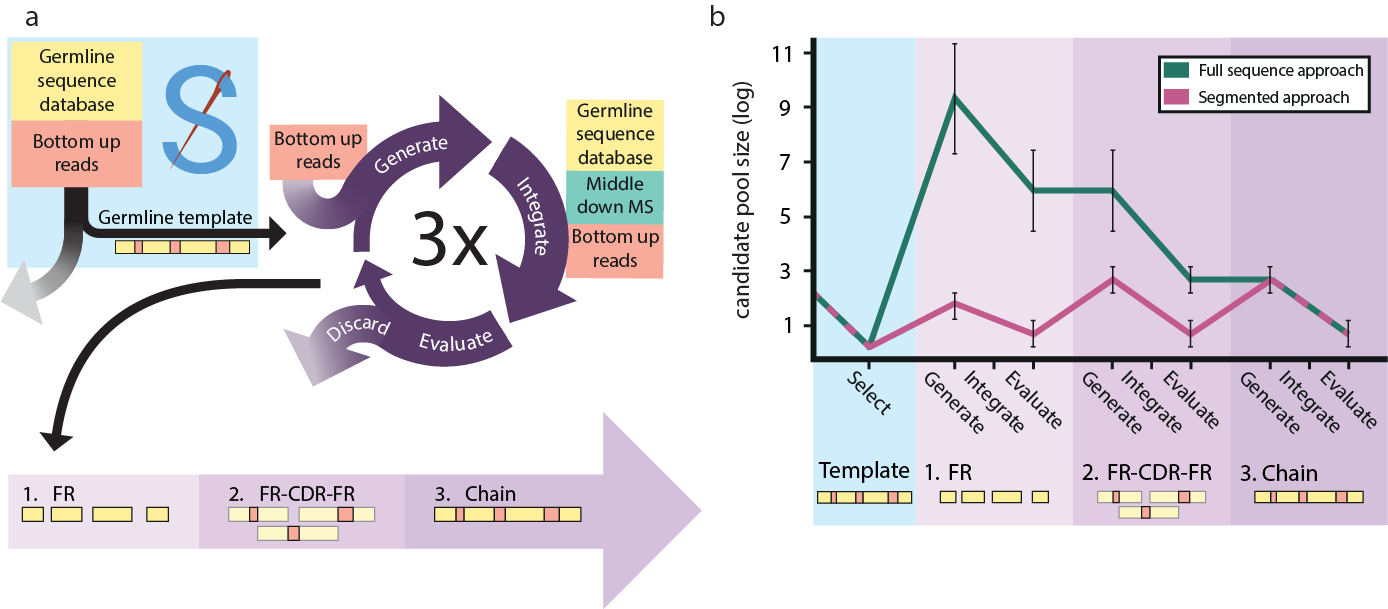
\includegraphics[]{Chapter.5/Figures/f1.png}
  \caption{\textbf{Modular sequencing can be used to limit the search space.} ~~a) Schematic of data-integration workflow. The approach consists of three stages in which increasingly large sequence segments are sequenced and then used as input for the next stage. Initially, only the framework regions (FRs) are sequenced. Then the FR candidates are converted into extended FR-CDR-FR candidates (\emph{i.e.}, CDRs with adjacent FRs). Finally, the FR-CDR-FRs are recombined into full chain candidates. Each stage follows a flow starting with sequence candidate generation based on input data (“Generate”). These candidates are scored using multiple data streams (“Integrate”), then the best candidates are selected using these scores (“Evaluate”). ~~b) Size of the search space throughout the workflow. The approximate number of candidates is shown in the modular approach (pink) versus processing the whole sequence at once (teal). By first sequencing smaller segments, the search space can be kept relatively small. The segment candidate pool is expanded at the start of the stage and reduced after scoring. This ensures we never consider more than $\sim$10\textsuperscript{3} segment candidates at the same time, keeping computational cost in balance .}
  \label{fig:fig5.1}
\end{figure*}


\subsection{Target mass determination and sample characterization by using MD-MS}
\label{ch:mass-determ}
To characterize the complexity of the samples and determine the precursor masses of the target chains, we collected MD LC-MS/MS data for all samples. Our MD approach was performed according to previously published protocols (see \textbf{\autoref{ch:ig-capt}: Immunoglobulin capture and Fab generation}) \cite{bondt2021direct, bondt2021human}. These protocols yield Fab fragments by specifically cleaving the Fc portion of the heavy chain. The resulting Fab fragments were then reduced before LC-MS/MS analysis, to yield separated Lc and Fd chains. We then deconvoluted the MS1 spectra to assess the number of unique Lc and Fd masses in each sample (\textbf{\autoref{fig:fig5.2}})
\begin{figure*}[!htb]
  \center
  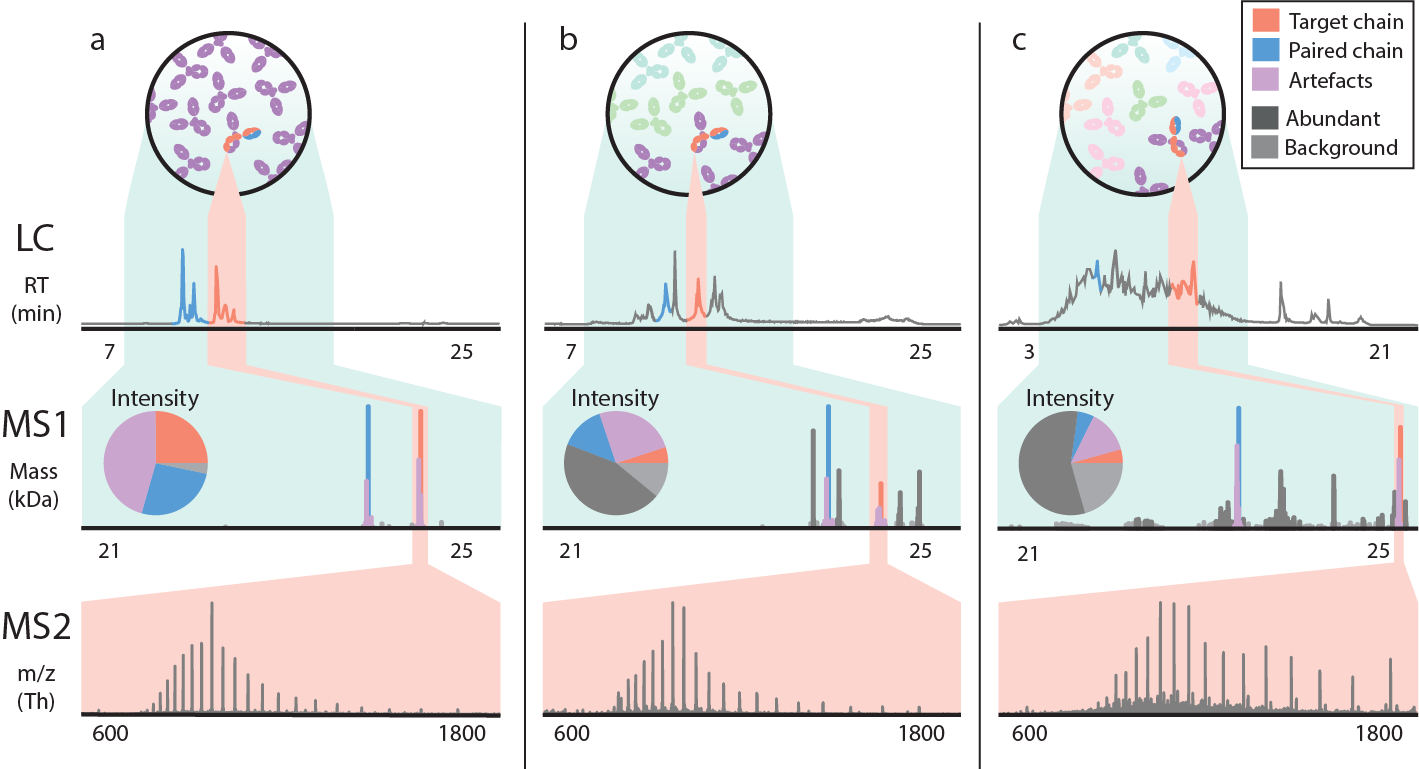
\includegraphics[]{Chapter.5/Figures/f2.png}
  \caption{\textbf{Increasing complexity leads to an increase in ambiguity in mass determination in middle-down proteomics of antibodies.} LC-trace (top panel), zero-charge deconvoluted mass spectrum (middle panel), and averaged MS2 spectrum (bottom panel). ~~a) Pure Trastuzumab with clear signals for the light chain and the Fd chain. ~~b) Mixture of Trastuzumab and two other monoclonal antibodies. ~~c) Polyclonal sample from plasma. The contributions of the target and paired chains diminish relatively when the background becomes more complex.}
  \label{fig:fig5.2}
\end{figure*}

For the monoclonal sample, as expected, 2 highly abundant peaks were observed (originating from the separated Lc and Fd chains), accounting for over half of the total deconvoluted intensity. When adjacent peaks in both mass and retention time (±50 Da and ±1 minute) are considered, this increases to over 90\% with the remaining masses consisting of background peaks of less than 5\% relative abundance (\textbf{\autoref{fig:fig5.2}a}). For the mixture of 3 mAbs, likewise and as expected, six abundant peaks were observed. The abundance of the target chains (±50 Da and ±1 minute) made up $\sim$33\% of the deconvoluted intensity. The other clones make up a total of 50\% of deconvoluted intensity and $\sim$20\% is background (\textbf{\autoref{fig:fig5.2}b}). Lastly, for the polyclonal sample, the target clone (±50 Da and ±1 minute) made up less than 20\% of deconvoluted intensity (\textbf{\autoref{fig:fig5.2}c}). The data in \textbf{\autoref{fig:fig5.2}} highlight challenges in deconvoluting MD-MS spectra. We observe that the deconvolution software reports (inaccurate) masses  besides the expected masses, increasingly so for more complex samples. To obtain the most exact masses, we averaged the MS1 spectra recorded over the elution window of each target chain (\textbf{\autoref{fig:fig5.2}}; highlighted in red) before deconvolution. This improved the mass assignments to within 30 ppm accuracy for the Trastuzumab Fd in the monoclonal and mix sample and yielded a target precursor mass of 24811.17 Da for the most abundant clone in the polyclonal sample extracted from serum. Similarly, the MS2 fragmentation spectra were averaged over the elution windows of the target chains and deconvoluted. This yielded 919, 265 and 469 deconvoluted fragment ion peaks for the monoclonal, mix and polyclonal sample respectively (\textbf{\autoref{tab:tabs5.1}}  ).


\subsection{Using multi-enzyme shotgun proteomics data for \emph{de novo} sequencing}
\label{ch:bu-ms}
As part of the analysis each sample was also measured by BU-MS, by digesting each sample with 4 proteases in parallel and collecting peptide-centric LC-MS/MS data. The resulting spectra were submitted for \emph{de novo} peptide identification using PEAKS \cite{ma2003peaks:}, yielding a total (\emph{i.e.}, cumulatively from all protease treatments) of 14000, 27421 and 35003 \emph{de novo} peptide reads for the monoclonal sample, the mixture of three, and the polyclonal sample, respectively (\textbf{\autoref{tab:tabs5.1}}). To illustrate the growing challenges of sequencing through shotgun proteomics in more complex samples, we reconstructed the known sequence of the Trastuzumab Fd from the \emph{recombinant benchmark samples} (\emph{i.e.}, the monoclonal and mixture of three sample) using BU-MS data alone. To this end, the peptide reads for these samples were submitted to the \emph{de novo} peptide assembly tool Stitch \cite{schulte2022template-based}. The resulting output for the monoclonal sample was nearly perfect (\textbf{\autoref{fig:fig5.3}a}). However, the consensus sequence as obtained for the sample from the mixture of 3 mAbs contained 4 erroneous residue predictions in the FR2, and 6 in the CDR1 and CDR2 (\textbf{\autoref{fig:fig5.3}c}). These errors were the result of low peptide coverage, caused by assigning reads to the wrong templates. This caused splitting of reads that belonged to the same chain. Furthermore, the unassisted germline recombination by Stitch failed to select the correct V-region for recombination, as it was not the highest scoring V-region in the mix sample. This standard \emph{de novo} sequencing of a recombinant mAb, already becomes difficult when two other mAbs of equal abundance are spiked into the sample.
\begin{figure*}[!htb]
  \center
  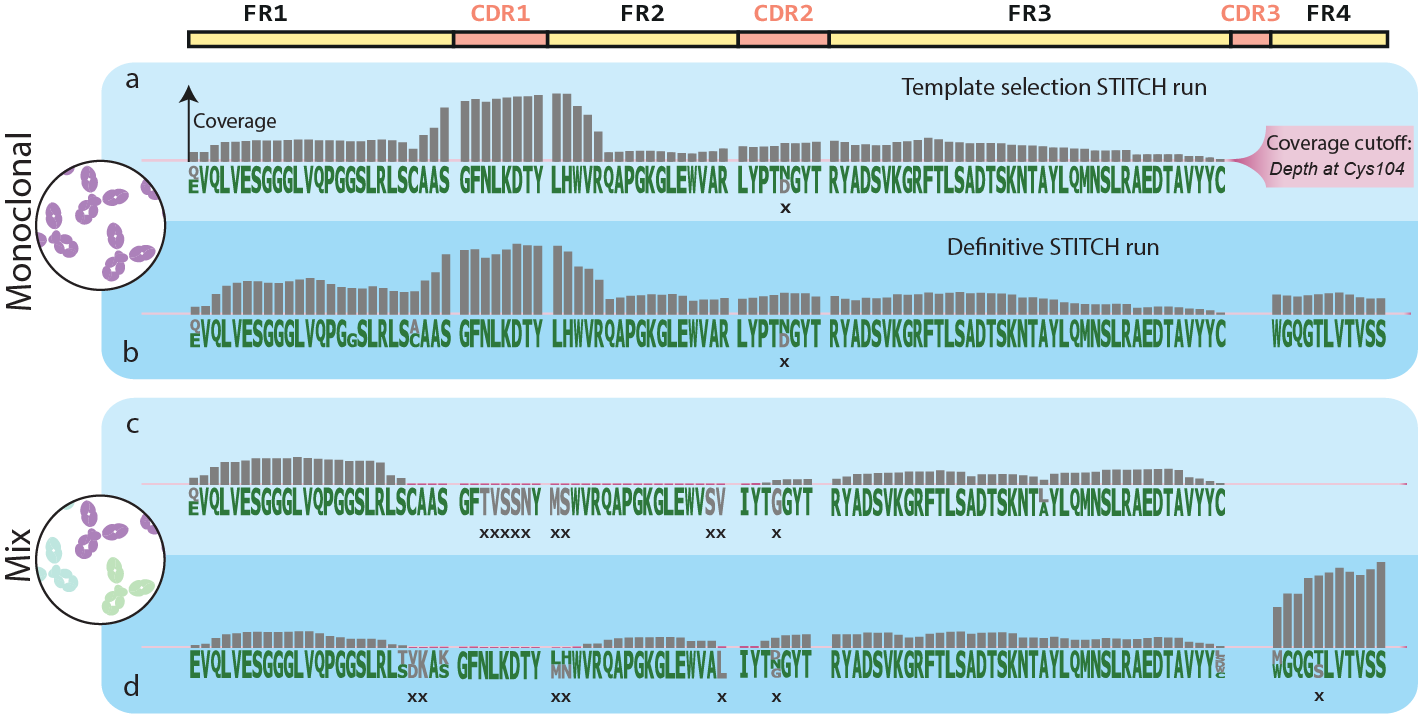
\includegraphics[]{Chapter.5/Figures/f3.png}
  \caption{\textbf{Sequencing higher complexity samples lead to a loss of fidelity in sequencing when using only shotgun proteomics data.} Sequencing results for the monoclonal (panel a-b) and mixture of 3 mAbs (panel c-d) samples are shown. Each sample was submitted to Stitch twice: as a \emph{template selection} run (light blue, panel a and c) and a \emph{definitive} run (dark blue, panel b and d). Each panel shows residue candidates as letters and depth of coverage as bars. The monoclonal sample had no coverage below the cut-off (pink highlight), very few erroneous residue candidates (grey residues), ambiguity, or errors in the consensus sequence (marked with “\emph{x}”). The mixture of 3 mAbs sample had substantially more stretches of sequence with low coverage (pink bars), resulting in more ambiguity, erroneous candidates, and errors.}
  \label{fig:fig5.3}
\end{figure*}

To tackle these issues, we ran Stitch again with refined templates (\emph{i.e.} the consensus sequence as output by the initial Stitch run, or \emph{template selection} run, rather than the germline sequence) and a lower score cut-off for the input reads (50 instead of 85). To ensure recombination of the correct V-region, we manually defined which V-region templates should be recombined by Stitch by providing refined templates equal to the number of abundant clones present in the MD data (1 and 3 for the monoclonal and mixture sample, respectively; \textbf{\autoref{fig:fig5.2}a and b}). For the monoclonal sample we selected the best scoring V-region, IGHV3-66, as a refined template. For the sample of 3 mAbs we selected 3 V-region templates: the highest unique score (IGHV4-39), the highest score (IGHV4-30-4), and the highest score in a different family (IGHV3-66). This additional Stitch run, or \emph{definitive} run, gave a major improvement for analysis of Trastuzumab in the 3 mAb sample, as it improved the depth of coverage 2 to 28-fold and raised depth of coverage above the dynamic cut-off (the depth of coverage at Cys104, \textbf{\autoref{fig:fig5.3}}) for 13 out of 21 positions (\textbf{\autoref{fig:fig5.3}d}). Pleasingly, these adjusted settings had no detrimental effects on the performance for the monoclonal sample (\textbf{\autoref{fig:fig5.3}b}), although some ambiguity remained in the predicted sequence for Trastuzumab in the 3 mAb sample.


\subsection{Integrating multiple evidence streams}

\subsubsection{Performance on recombinant samples}

\paragraph{Framework region sequencing}
\label{ch:fr}
Using the residue frequency tables (\textbf{\autoref{fig:figs5.1}}) from both Stitch runs, as well as a residue frequency table generated from the IMGT database, FR candidate sequences were generated by converting ambiguous residues into sequence candidates (\textbf{\autoref{fig:figs5.1}}). This yielded between 1 and 756 candidates per target FR (\textbf{\autoref{tab:tabs5.2}}) and included the known correct candidate for all recombinant benchmark samples. These candidates were evaluated against experimental BU- and MD-MS evidence and ranked by a combination of the resulting scores. For BU-MS scoring, a score was used that represents the depth of coverage of exact sequence matches longer than 6 residues, weighted by match length (termed Shotgun-score; \textbf{\autoref{tab:tabs5.3}}). For MD-MS scoring, a score was used that represents the overlap between theoretical fragments of the sequence and peaks in the MD fragmentation spectrum (MD-score; \textbf{\autoref{tab:tabs5.3}}). The MD-score is obtained using a \emph{sliding window} scoring algorithm, which slides theoretical fragments generated from a given (sub)sequence over the spectrum to find the best scoring position, and thus outputs the optimal prefix- and suffix- mass of a given contig (\textbf{\autoref{fig:figs5.2}}). Candidates missing highly conserved residues (Cys23, Cys104) as well as terminal segment (\emph{i.e.}, FR1 and FR4) candidates with illogical prefix- or suffix- masses were removed in a first pass filtering step. This reduced the candidate lists up to 10-fold, to a maximum of 90 candidates (\textbf{\autoref{fig:figs5.3}}).
We further filtered the candidate pools to a maximum of 40 candidates (\textbf{\autoref{tab:tabs5.2}}) without eliminating any correct candidates by manual inspection of the scores. For the monoclonal sample, the correct FR1 candidate was ranked \#1 with a large discrepancy between scores (\textbf{\autoref{fig:figs5.3}}). As FR2, FR3, and FR4 only had one candidate each, no selection was needed. However, it was encouraging to see that the sliding window algorithm was able to correctly determine the prefix masses for these contigs with a mass error that did not exceed 18 ppm.
The candidate pools for the mixture of 3 mAbs were reduced from 240, 756, 5 and 4 candidates to 40, 7, 1 and 2 candidates for al FRs respectively (\textbf{\autoref{tab:tabs5.2}}). For FR1, we rejected 200 candidates in the first pass, leaving 40 candidates. No further filtering was possible, as fragment and read coverages were too low for confident filtering (maximum of 2 fragments and no read coverage past Cys23). The FR2 candidates had many overlapping scores (\textbf{\autoref{fig:figs5.3}}) due to low read coverage of the N-terminal ambiguous residues (\textbf{\autoref{fig:fig5.3}c and d}) and a near total overlap of theoretical fragments for these candidates. We rejected the lower MD-scores (106 vs 121), which represented the same fragments but without a fragment match on the second residue. This reduced the number of candidates from 756 to 90. Subsequent filtering using the Shotgun-score, rejecting all but the best Shotgun-score (9.4k), left only 7 candidates, representing a single remaining ambiguous N-terminal residue. For FR3, only 1 out of 5 candidates had the highly conserved Cys104, leading us to reject all other candidates. For FR4, we rejected all candidates not starting with the conserved Trp118 but considered the difference in Shotgun-score for the remaining 2 candidates too small to reject either.

\paragraph{Complementarity determining region sequencing}
\label{ch:cdr}
To determine the sequence of the CDRs, we extended the selected FR candidates into FR-CDR-FR candidates. All adjacent FR candidates were paired to obtain all possible neighbouring pairs. We then calculated the mass gap between each of these FR pairs (which is equal to the theoretical molecular weight of the CDR sequence) using the prefix- and suffix- mass of each FR candidate. Each FR pair was converted into a set of FR-CDR-FR candidates by connecting the FRs with candidate CDR sequences. These candidate CDR sequences were generated by first connecting peptide reads that extend from the FRs into the CDR, then discarding the candidates that do not match the calculated molecular weight of the CDR at 5 Da tolerance (\textbf{\autoref{fig:figs5.4}}). The resulting FR-CDR-FR candidates were scored and ranked using the MD- and Shotgun- score (\textbf{\autoref{tab:tabs5.3}}).
The top 10 FR-CDR-FR candidates for each FR pair were manually evaluated based on the scores to select the most likely FR-CDR-FR candidates. For both recombinant benchmark samples, these candidates contained the correct sequence for CDR1, CDR2 and CDR3. For the monoclonal sample, 10 FR-CDR-FR candidates were generated per CDR (\textbf{\autoref{tab:tabs5.2}}). The correct candidate for each CDR could easily be selected using the Spectrum and Shotgun-score (\textbf{\autoref{fig:figs5.2}}). The selected candidates all had the top MD-score (255, 508 and 1561 for the CDR1, CDR2 and CDR3 respectively) and the best (CDR1 and CDR2) or second best (CDR3) Shotgun-score (137k, 56k and 122k respectively).
For the mixture of 3 mAb sample 1106, 49 and 20 FR-CDR-FR candidates were generated for the CDR1, CDR2 and CDR3, respectively (\textbf{\autoref{tab:tabs5.2}}). Despite the much larger starting pools, the correct CDR1- and CDR2- candidates could be selected unambiguously during manual inspection as they had the second best and best MD-scores (143 and 257 for CDR1 and CDR2 respectively) and the top Shotgun-score (30k and 40k respectively; \textbf{\autoref{fig:figs5.3}}). The selected FR-CDR-FR candidates for CDR1 also caused rejection of the remaining incorrect FR1 and FR2 candidates, which left only 7 FR-CDR-FR candidates for CDR2 as the rest did not contain the right FR2.
Scoring for the CDR3 was more ambiguous. Fragment coverage was insufficient to make a distinction between the FR-CDR-FR candidates, as MD-scores ranged only from 280 to 282. The Shotgun-scores were distributed in two clusters based on which FR4 candidate was included (\textbf{\autoref{fig:figs5.3}}). The correct FR4 (starting with WGQGT) scored $\sim$221k while the incorrect FR4 (starting with WGQGS) scored higher ($\sim$244k). However, we noted that the candidates with the wrong FR4 lacked connecting reads between the FR4 and CDR3. The candidates with the correct FR4 sequence had fewer but longer and more overlapping reads which connected the CDR3 and FR4 better (average read length of $\sim$25 vs average read length of $\sim$12). We rejected the higher Shotgun-scores on this basis.
The candidate pool with the correct FR4 included 2 incorrect FR-CDR-FR candidates, SR\textbf{\emph{WNDG}}FYAMDY and SR\textbf{\emph{DNWG}}FYAMDY, that were nearly identical to the correct candidate, SR\textbf{\emph{WGGDG}}FYAMDY. We selected these 3 candidates based on the presence of longer and more overlapping reads in the CDR3 than the other 7, same as above. However, we could not discriminate between the 3 isobaric candidates at this point, leaving 3 candidates for the CDR3.


\paragraph{Full chain sequencing}
We next expanded the scope to the entire target chain to verify the selected FR-CDR-FR candidates. To achieve this, we recombined all remaining FR1 to FR4 candidates and transformed these FR-sets into full length chain candidates by joining the FRs with CDR candidates in the same manner as before (see \textbf{\autoref{ch:cdr}: Complementarity determining region sequencing}; \textbf{\autoref{fig:figs5.4}}). The resulting chain candidates that deviated more than 5 Da from the precursor mass in the MD-MS data were discarded. To ensure that the selected FR-CDR-FR candidates indeed represented the best predictions, all resulting chain candidates were scored and ranked using the MD- and Shotgun- score (\textbf{\autoref{fig:figs5.3}}).
This recombination yielded 930 chain candidates for the monoclonal sample and 616 for the mixture of 3 mAb sample. The correct chain candidate for the monoclonal sample was ranked \#1, despite not having the highest Shotgun-score (267k vs 270k) or MD-score (1815 vs 1818). For the mixture of 3 mAb sample, the chain candidates made up solely out of previously selected FR-CDR-FR candidates were ranked \#3-5, with the correct sequence at \#5. The top 2 candidates had CDR3 sequences that were previously rejected in the CDR sequencing stage, which were again rejected on the same basis (shorter, less overlapping reads). The isobaric CDR3s still could not be confidently ranked as the scores were too close, with Shotgun-scores between 255.7k and 255.8k and MD-scores between 426.1 and 427.2 (\textbf{\autoref{fig:figs5.3}}). Low fragment coverage combined with other clones being present at similar concentrations seemingly prevented us from resolving the final ambiguities for the mix sample. This is highlighted by the large difference between the MD-scores for the correct chain candidates (426 for the mix sample vs 1815 for the monoclonal sample).


\subsubsection{Performance on the complex polyclonal samples}
After successfully reconstructing the known sequence of Trastuzumab from the recombinant samples, we proceeded to analyse the polyclonal sample. We selected the most abundant heavy chain (precursor mass 24811.17 Da; \textbf{\autoref{tab:tabs5.1}}) as a sequencing target and prepared deconvoluted fragmentation spectra from the raw MD-MS data (see \textbf{\autoref{ch:mass-determ}: Target mass determination and sample characterization using MD-MS}; \textbf{\autoref{fig:fig5.2}c}). To generate FR candidates for the selected target chain, we submitted \emph{de novo} peptide reads to Stitch (see \textbf{\autoref{ch:bu-ms}: Using multi-enzyme shotgun proteomics data for \emph{de novo} sequencing}). From the \emph{template selection} run we selected IGHV3-33, the most abundant V-region in the Stitch results, for recombination during the \emph{definitive} run (\textbf{\autoref{fig:fig5.4}a}). The Stitch frequency tables from both runs were then converted into FR candidates as described above (see \textbf{\autoref{ch:fr}: Framework region sequencing}; \textbf{\autoref{fig:figs5.1}}).
\begin{figure*}[!htb]
  \center
  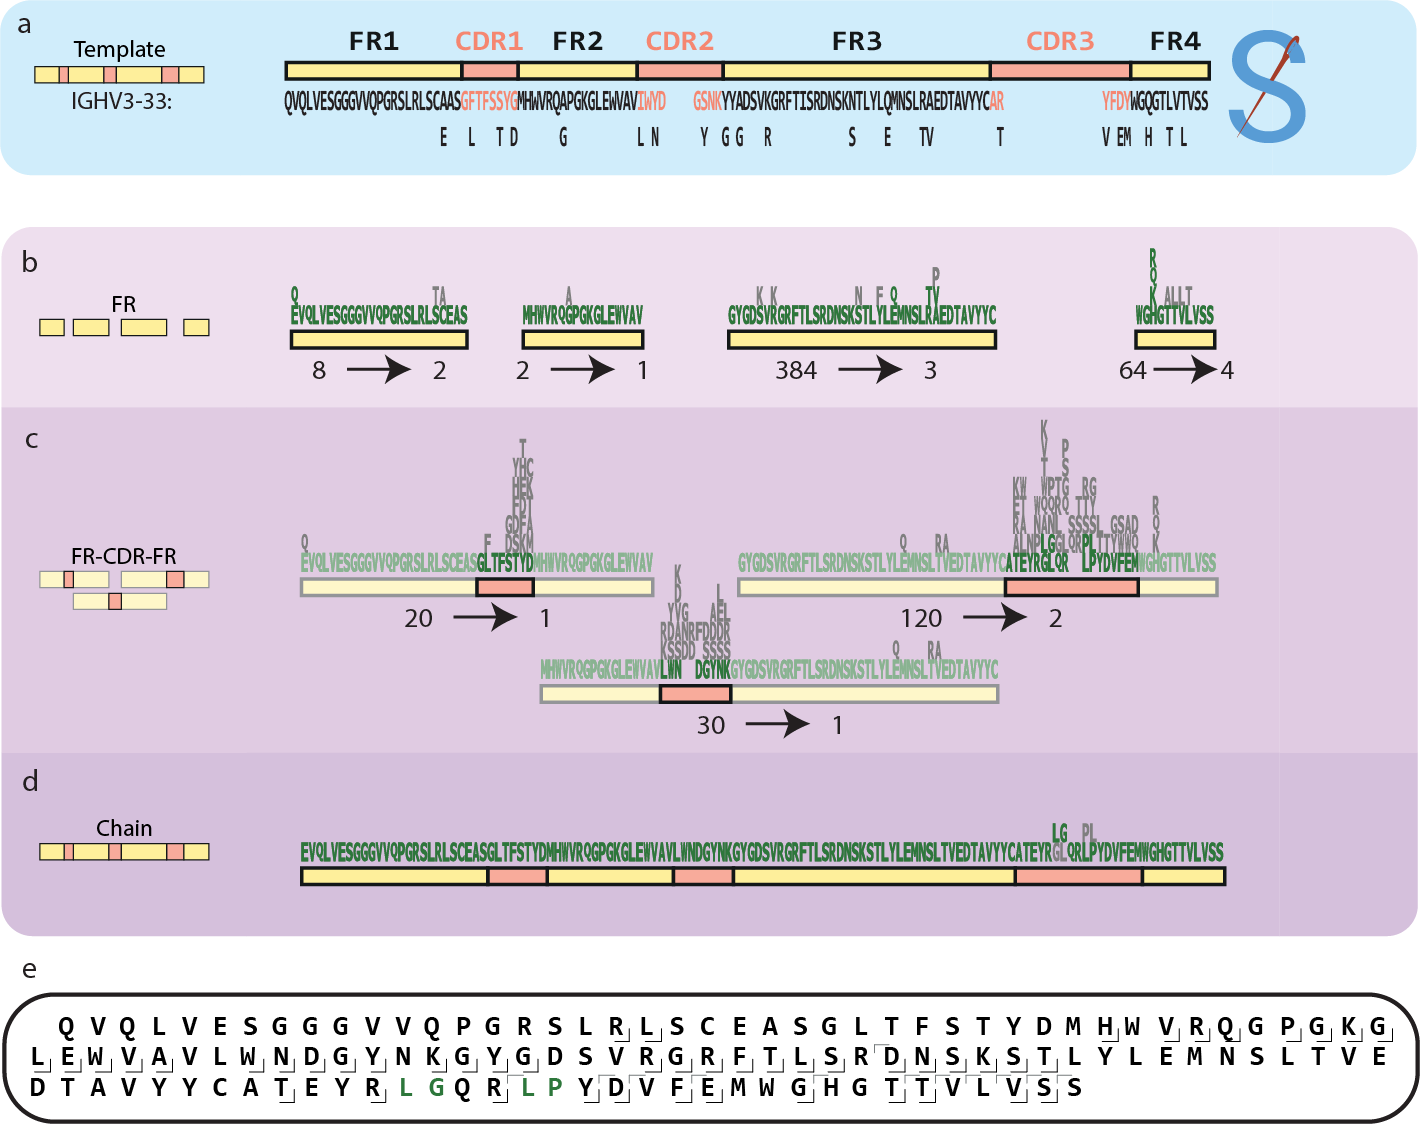
\includegraphics[]{Chapter.5/Figures/f4.png}
  \caption{\textbf{Sequencing an abundant IgA1 heavy chain in a polyclonal sample converges on a single sequence prediction.} The sequencing process of the target chain in the polyclonal sample is shown. Residue candidates per position are shown in sequence logos, with rejected residue candidates in grey. Below the sequence logos the number of candidates at the start and end of the stage is shown. ~~a) The selected germline template, IGHV3-33*06, is shown along with the deviations from the final sequence. ~~b) In the FR sequencing stage, we reduced all FR candidate pools to 4 candidates or less despite starting with large pools of FR3 and FR4 candidates. ~~c) During the CDR sequencing stage, we converged on a single CDR1 and CDR2 candidate, thereby also rejecting the remaining incorrect FR1 and FR3 candidates. The only remaining ambiguity was in between two isobaric CDR3 sequences. ~~d) Recombining the remaining FR candidates into chain sequences yielded 975 chain candidates. Two of these contained the previously selected CDRs. These two candidates were isobaric, had highly similar Shotgun-scores and fully overlapping fragment coverage. ~~e) middle-down fragment coverage for the final sequence (constant region not shown).}
  \label{fig:fig5.4}
\end{figure*}

FR candidate generation yielded 8, 2, 384 and 64 candidates for the FR1 to FR4 respectively. After scoring and filtering this was reduced to 2, 1, 3 and 4 candidates (\textbf{\autoref{fig:fig5.4}b}, \textbf{\autoref{tab:tabs5.2}}). From the FR candidates which remained after the first pass (see \textbf{\autoref{ch:fr}: Framework region sequencing}; \textbf{\autoref{tab:tabs5.2}}), we rejected all but the top scoring candidates with respect to MD-score (10, 155, 163 and 133 for FR1 to FR4 respectively; \textbf{\autoref{fig:figs5.3}}). We then manually selected candidates for each FR based on Shotgun-score. For FR1, we selected the top 2 candidates (34k and 35k Shotgun-score) as the other two candidates had an LTC motif that had a lower Shotgun-score. This left a single ambiguous isobaric residue, an N-terminal pyro-Q/E. For FR2, only 1 candidate had the top MD-score, which was much higher than the alternative candidate (155 vs 105). For FR3 the top 3 Shotgun-score candidates were selected (27k-30k), leaving 2 ambiguous sites (Q/E and TV/RA, \textbf{\autoref{fig:fig5.4}b}). For FR4, the top 4 candidates in terms of Shotgun-score (308k-310k) were selected, representing a single ambiguous N-terminal residue (\textbf{\autoref{fig:fig5.4}b}).
Using these FR-candidates, 20, 30 and 120 FR-CDR-FR candidates were generated for CDR1 to CDR3 respectively. The top MD- and Shotgun-scores were unambiguous for CDR1 and CDR2 (\textbf{\autoref{fig:figs5.3}}), identifying the CDR1 as GLTFSTYD (MD-score 118, Shotgun-score 57k), and CDR2 as LWNDGYNK (MD-score 377, Shotgun-score 51k). By selecting these FR-CDR-FR candidates, 2 out of 3 remaining FR3 candidates could be rejected leaving 40 FR-CDR-FR candidates for CDR3. From these, we selected 2 isobaric FR-CDR-FR candidates (\textbf{\emph{LG}}QR\textbf{\emph{PL}} and \textbf{\emph{GL}}QR\textbf{\emph{LP}}) with the top Shotgun-scores (346.2k and 346.4k) and the second-best MD-score (both 370.7) (\textbf{\autoref{fig:fig5.4}c}, \textbf{\autoref{fig:figs5.3}}).
Recombining the selected FR candidates into chain candidates yielded 975 chain candidates. Two chain candidates were made up of previously selected FR-CDR-FR candidates and scored very well as they had the fourth highest MD-score (434) and top Shotgun-scores (411k; \textbf{\autoref{fig:figs5.3}}). To resolve the remaining ambiguity in the CDR3 (\textbf{\autoref{fig:fig5.4}d}), we revisited the peptide coverage for this region. This revealed a break in the peptide coverage of CDR3 in one of the candidates suggesting the CDR3 sequence LGQRPL. However, strong support for the LP motif in the CDR3 led us to reinspect the \emph{de novo} reads manually, where we found several reads suggesting the CDR3 sequence LGQRLP, a sequence absent in any single bridging or overhanging CDR3 reads. Rescoring this sequence indeed revealed an increased Shotgun-score, from 411.3k to 411.7k, providing the final piece of the sequence (\textbf{\autoref{fig:fig5.4}e}).


\section{Discussion}
With this work we show that integration of BU and MD data is beneficial to achieve a higher fidelity for \emph{de novo} extraction of the sequences of antibodies. To provide a solid basis with the \emph{de novo} peptide data, we utilize Stitch \cite{schulte2022template-based} although this step does not yet allow for unambiguous sequence determination. To correct the errors and resolve this ambiguity, MD fragmentation data was used. Although the MD data for even the most abundant clone in a mixture is far from complete, we show that it can be used as a potent filter to remove erroneous candidates and even to assist with filling gaps in the sequence. We have used the presented workflow to simultaneously sequence light and heavy chains, but for the sake of brevity have omitted the light chain sequencing efforts in this manuscript. As we analyse one chain at a time, there is little difference between the analysis of light and heavy chains aside from differences arising from the quality of the data or the complexity of the target. Light chains are less complex owing to a lower degree of somatic hypermutation and the lack of a D-segment. Unsurprisingly therefore, these targets performed equally well or better than their heavy chain counterparts.
The polyclonal sample used in this study still represents a hand picked case for sequencing plasma antibodies, where the sample was dominated by a single clone. While moving to more complex samples will surely pose new challenges, it has been shown that circulating antibody repertoires are, more often than previously thought, dominated by a limited number of clones \cite{bondt2021human, bondt2021direct}. We are therefore optimistic that the presented approach will be applicable to a significant fraction of polyclonal samples . Additionally, for those samples where it does fall short due to sample complexity, enrichment strategies can be applied before analysis in an effort to reduce sample complexity and increase the chance of successfully obtaining the protein sequence. Another point to improve is the need for expert manual interpretation at various points in this workflow, which significantly limits the throughput. Although the main goal of the presented work was to define a broadly applicable protocol for polyclonal antibody sequencing, we have not yet been able to define robust score cut-offs for several decision points making this an intermediate step in the development of a fully automated pipeline. The integration of multiple data sources, as well as the diversity of the analysed samples (polyclonal, complex), targets (light or heavy chain, dominant clones, isotypes and subclasses), regions (FR1-4, CDR1-3) and segments (FRs, FR-CDR-FR, chain), makes this an even bigger challenge. As the field matures however, a point will be reached where scoring functions and corresponding cut-offs can be defined. This will automate an ever-increasing portion of this work, eventually leading to a high throughput, fully automated method.


\section{Materials and Methods}

\subsection{Immunoglobulin capture and Fab generation}
\label{ch:ig-capt}

\subsubsection{Recombinant IgG1 sample preparation}
The IgG purification and generation of IgG1 Fabs for the recombinant monoclonal and mix samples was performed as previously published \cite{bondt2021human}. IgGs were captured using CaptureSelect FcXL affinity matrix (Thermo Scientific). Mobicol spin filters were assembled according to manufacturer instructions and placed in 2 mL Eppendorf tubes. Then 20 µL FcXL affinity matrix slurry was added to the spin filter, followed by three washing steps with 150 µL PBS, in which the liquid was removed by centrifugation for 1 min at 1000 × \emph{g}. Two additional washing steps with 150 µL were performed. The affinity matrix was resuspended in 150 mL PBS, and 100 µg of sample was added. The samples were then incubated while shaking for one hour. Next, the flow-through was collected and the affinity matrix with bound IgGs was washed four times with 150 µL PBS. bound IgGs were digested overnight using 50 µL PBS containing 100 U of the IgdE protease (FabALACTICA®, Genovis, Llund, Sweden) on a thermal shaker (Eppendorf, The Netherlands) at 37 °C. Next, 10 µL of Ni-NTA beads were added to bind and remove the His-tagged protease and left incubating for an additional 30 minutes. The flow through after centrifugation contained the IgG1 Fab fragments generated.

\subsubsection{Serum IgA1 sample preparation}
The IgA purification and generation of IgA1 Fabs for the polyclonal sample was performed as previously published \cite{bondt2021direct}. IgAs were captured from a patient serum sample using CaptureSelect IgA affinity matrix (Thermo Scientific). 40 µL bead slurry was added directly to Pierce spin columns with screw cap (ThermoFisher Scientific). The beads were then repeatedly washed with 150 µL PBS by centrifugation at 500 × g, room temperature (RT). After the third wash, a plug was inserted to the bottom of the individual spin columns and 100 µL PBS was added to the beads. Twenty microliter of serum was diluted in 150 µL PBS and added, then incubated for 1 hour while shaking. Following the incubation, the plugs were removed from the spin columns and the diluted sample was collected by centrifugation for 1 min at 500 × g, RT. Then the beads were washed four times by addition of 200 µL PBS and subsequent centrifugation for 1 min at 500 × g, RT. After the fourth wash the plugs were reinserted into the bottom of the spin columns. We added to each spin column 50 µL PBS containing 40U SialEXO (SialEXO, Genovis, Llund, Sweden), a sialidase cocktail to remove sialic acids from the O-glycans, and incubated for 1 h at 37°C with continuous shaking at 750 rpm. 1 µL (40 U) of OgpA enzyme (OpeRATOR, Genovis, Llund, Sweden) was then added, and incubation was continued overnight, in and Eppendorf thermal shaker. Next, 10 µL of Ni-NTA beads were added to bind and remove the His-tagged proteases and left incubating for an additional 30 minutes. The flow through after centrifugation contained the IgA1 Fab fragments generated.

\subsection{Bottom-up \emph{de novo} sequencing}

\subsubsection{Sample preparation}
Fab fragments were digested for BU analysis as described previously \cite{bondt2021human}. All purified Fab antibody fragments were dried under vacuum and resuspended in a 50 mM aqueous ammonium bicarbonate buffer. For each bottom-up analysis, 12 µg of sample was used, 3 µg per protease. For digestion with trypsin, chymotrypsin, elastase and thermolysin, a sodium deoxycholate (SDC) buffer was added to a total volume of 80 µL, 200 mM Tris pH 8.5, 10 mM TCEP, 2\% (w/v) SDC final concentration. For digestion with pepsin, a urea buffer was added to a total volume of 80 µL, 2M urea, 10 mM TCEP. Samples were denatured for 10 min at 95 °C followed by reduction for 20 min at 37 °C. Next, iodoacetic acid was added to a final concentration of 40 mM and incubated in the dark for 45 min at room temperature for alkylation of free cysteines. Then for trypsin, chymotrypsin and thermolysin, 50 mM ammonium bicarbonate buffer was added to a total volume of 100 µL. For pepsin 1 M HCl was added to a final concentration of 0.04 M. A total of 0.06 µg of each protease was added and the mixture incubated for 4 hours at 37 °C. After digestion 2 µL formic acid was added to precipitate the SDC. SDC was removed by centrifugation for 20 min at maximum speed (20817 × \emph{g}) after which the supernatant was moved to a new tube. The final samples were desalted by Oasis HLB (Oasis).  Sorbent was wetted using 2x 200 µL ACN, followed by equilibration with 2x 200 µL water/10\% formic acid.  The sample was loaded and washed with 2x 200 µL Mili Q water/10\% formic acid.  Finally, the sample was eluted using 2x 50 µL water/50\% ACN/10\% formic acid and dried down by vacuum centrifuge. Prior to MS analysis samples were reconstituted in 2\% FA.

\subsubsection{LC-MS/MS}
Data acquisition was performed on the Orbitrap Fusion Tribrid Mass Spectrometer (Thermo Scientific, San Jose, CA, USA) coupled to UHPLC 1290 system (Agilent Technologies, Santa Clara, CA, USA) as previously published \cite{bondt2021human}. Briefly: Peptides were trapped (Dr. Maisch Reprosil C18, 3 mm, 2 cm3 100 mm) prior to separation (Agilent Poroshell EC-C18, 2.7 mm, 500 mm 3 75 mm). Trapping was performed for 10 min in solvent A (0.1\% HCOOH in Milli-Q), and the gradient was as follows: 0 – 13\% solvent B (0.1\% HCOOH in 80\% CH3CN) over 5 min, 13 – 44\% solvent B over 65 min, 44 – 100\% solvent B over 4 min, and 100\% B for 4 min (flow was split to achieve the final flowrate of approximately 200 nL/min). MS data was collected in a data-dependent fashion with survey scans ranging from 350-2,000 Th (resolution of 60,000 @ \emph{m/z} 200), and up to 3 sec for precursor selection and fragmentation with either stepped higher-energy collisional dissociation (HCD) set to [25\%, 35\%, 50\%] or electron transfer dissociation (ETD), used with charge-normalized settings and supplemental activation of 27\%. The MS2 spectra were recorded at a resolution of 30,000 (@ \emph{m/z} 200).

\subsubsection{Data analysis}
Bottom-up MS/MS spectra were processed with the PEAKS-X \emph{de novo} sequencing suite (Bioinformatics Solutions Inc., Waterloo, ON, Canada). Default settings were used unless explicitly mentioned. Variable modifications were set to pyro-Glu from E, pyro-Glu from Q, oxidation (H/W), oxidation ~~m) . Max 4 variable modifications per peptide, max 5 peptides reported per spectrum, 0.02 fragment mass error tolerance, 20 ppm parent mass tolerance, fixed modification: Carboxymethyl. The resulting \emph{de novo} predictions (referred to as \emph{reads} throughout the manuscript), were inserted into the proteomic short read assembly tool Stitch for two subsequent runs to yield a frequency table and select a germline sequence template for each target chain. The residues of this sequence template were numbered according to the IMGT numbering convention \cite{lefranc1997unique}. The \emph{de novo} reads were numbered by aligning them to the sequence template using the Smith Waterman algorithm with a custom scoring matrix (Supplementary data 1) and copying the numbering. Throughout the manuscript, AA residues are referred to by their IMGT numbering.

\subsubsection{Germline database preparation}
The full IMGT database was used as a source of homologous germline sequences (Supplementary data 2). This database was filtered by excluding non-human entries, entries with identical sequences, partial or non-functional entries and sequences including wildcards or non-canonical AAs. The resulting sequences were filtered by excluding allelic polymorphisms to create a reduced and nonredundant set of germline template sequences, as described previously \cite{schulte2022template-based}. Only the constant regions relevant to the analysed sample were included (\emph{i.e.}, IgA1 for the polyclonal sample and IgG1 for the monoclonal and mix samples). These constant regions were cleaved to match the Fab fragments produced by the IgdE and OgpA enzymes. The resulting template sequences were used by Stitch for template selection and read assembly, and to generate the IMGT residue frequency table used for FR generation (\textbf{\autoref{fig:figs5.1}}).

\subsection{Middle-down \emph{de novo} sequencing}

\subsubsection{LC-MS/MS}
All Fab samples were denatured and reduced in 10 mM tris(2-carboxyethyl)phosphine (TCEP) at 60 °C for 30 min prior to LC-MS/MS analysis. For each LC-MS/MS experiment 2-5 µg of sample was injected. Reversed-phase liquid chromatography was performed by using a Thermo Scientific Vanquish Flex UHPLC instrument (Thermo Fisher Scientific, Germering, Germany), equipped with a 2.1 mm x 50 mm or 1 mm x 150 mm MAbPac RP analytical column (Thermo Fisher Scientific, Germering, Germany) and directly coupled to an Orbitrap Fusion Lumos Tribrid mass spectrometer (Thermo Fisher Scientific, Bremen, Germany). The column preheater, as well as the analytical column chamber, were heated to 80 °C during chromatographic separation.
The recombinant samples were separated over 27 min at a flow rate of 250 µL/min. The polyclonal sample in 22 min at a flow rate of 150 µL/min. Gradient elution was achieved by using two mobile phases A (0.1\% HCOOH in Milli-Q HOH) and B (0.1\% HCOOH in CH3CN) and ramping up B from 10 to 25\% over one minute, from 25 to 40\% over 14 min, and from 40 to 95\% over one minute. MS data were collected with the instrument operating in Intact Protein and Low Pressure mode. The spray voltage was set at 3.3 kV, capillary temperature 350 °C, probe heater temperature 100 °C, sheath gas flow 15, auxiliary gas flow 5, and source-induced dissociation was set at 15 V.
The reduced Fab chains were analysed with a resolution setting of 120k (@ 200 \emph{m/z}) in MS1, which allows for more accurate mass detection of smaller proteins (< 30 kDa) with 250\% AGC target and a maximum injection time of 250-500 ms. For the recombinant samples, 2 µscans were acquired and averaged per MS1 scan, in a range of 500-3000 Th. For the polyclonal sample 5 µscans were averaged in a range of 600-2000 Th. Data-dependent mode was defined as two scans.
MS/MS scans were acquired with a resolution of 120k (@ 200 \emph{m/z}) and a maximum injection time of 500 ms. The ions of interest were mass-selected by quadrupole 2-10 Th isolation windows, depending on the sample complexity, and accumulated to the AGC target prior to fragmentation. Electron-transfer dissociation (ETD) was performed using the following settings: 16 ms reaction time, a maximum injection time of 200 ms, and an AGC target of 1e6 for the ETD reagent. For data-dependent MS/MS acquisition, the intensity threshold was set to 5e4. MS/MS scans were recorded in the range of 350-5000 Th using high mass range quadrupole isolation.

\subsubsection{Data analysis}
Following the MD LC-MS/MS data acquisition of the Fab fragments, MS1 features were retrieved from the generated RAW files using BioPharmaFinder 3.2 (Thermo Scientific). Deconvolution was performed using the ReSpect algorithm, deconvoluting averaged scans over a selected RT window where the target clone eluted (\textbf{\autoref{tab:tabs5.1}}). The output mass range for the fragment ions was set at 10 to 40 kDa. Charge states between 10 and 50 were included with a minimum of 6 and 10 adjacent charges for the low and high model mass respectively. No relative abundance or score threshold was used. The target mass was set to 25 kDa, the number of peak models to 1, with a shape of 2 and 2 (left/right). The peak detection minimum significance measure was set to 1 standard deviation and the peak detection quality measured was set to 95\%. The MS2 spectra over the selected retention time were deconvoluted to yield their protonated monoisotopic fragment masses using the Freestyles Xtract algorithm. The minimum charge was set to 1, the maximum charge was set to 50, no thresholds were set for the minimum number of detected charges and the relative abundance.

\subsubsection{Contig scoring and refinement using middle-down data}
Throughout the manuscript, we make use of a scoring algorithm to optimize contig placement for a given MD-MS fragmentation spectrum, which we termed the \emph{sliding window} scoring algorithm (\textbf{\autoref{fig:figs5.2}}). This algorithm slides a set of theoretical fragments generated from the provided sequence along a provided \emph{m/z} range, incrementing the fragment masses by a set increment (default 0.01 Th). To limit processing time, peaks in the spectra are binned and the number of non-empty bins are counted for each position. The top scoring positions (default: top 100) are then refined by incrementing by smaller step size while scoring with a more refined scoring function \cite{olsen2004improved}, and finally the best scoring position is returned. This enables error-tolerant scoring of (sub)sequences, even if the exact prefix- and suffix- mass (distance from the N- and C- termini respectively) is not known, for example for sequence candidates which are not connected to the N- or C- terminus. In addition to a score, it also returns the optimal prefix- and suffix- mass for the sequence, which is used to calculate the theoretical molecular weight of CDRs during CDR sequencing, by calculating the mass gap between adjacent FR candidates.


\section{Acknowledgements}
SCdG and AJRH acknowledge the Dutch Research Council (NWO) supporting this work via project number 15575.


\subsection{Data availability}
The MS proteomics data have been deposited to the ProteomeXchange Consortium via the PRIDE \cite{perez-riverol2022pride} partner repository with the dataset identifier PXD042757.\\
The software and source code are freely accessible at\\
https://github.com/Bdegraaf1234/FabLabPublic.

\subsection{Author contributions}
AJRH conceived the study, SCdG performed the data analysis, wrote the required code and prepared the manuscript, RAS supervised the coding and prepared the manuscript, DS prepared the manuscript, AB performed the immunoglobulin capture, ST recorded and analysed the middle-down proteomics data, MH and WP recorded and analysed all shot-gun proteomics data.


\clearpage
\begin{subappendices}
  \beginsupplement


  \section{Supplementary material}
  Supplementary data as well as the source code can be found online at\\
  https://github.com/Bdegraaf1234/FabLabPublic

  \begin{table*}[!hbt]
    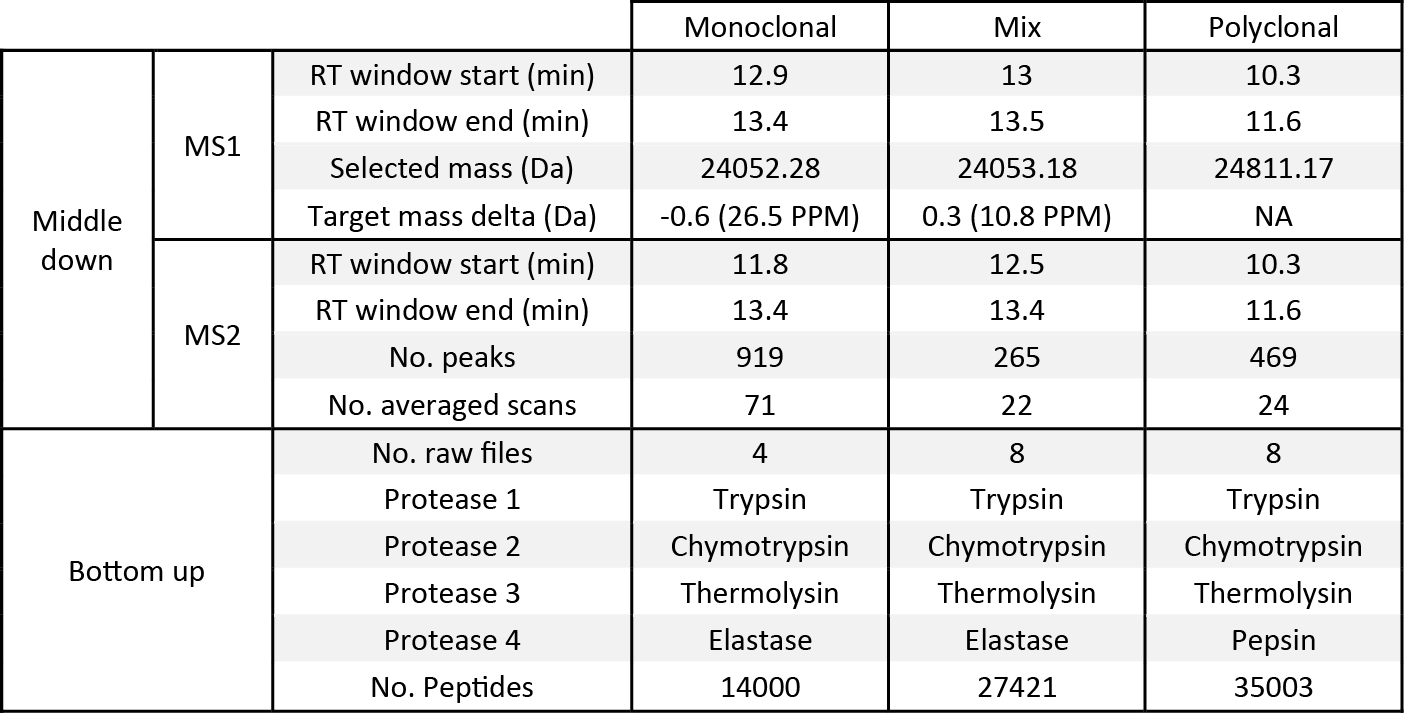
\includegraphics[]{Chapter.5/Figures/ts1.png}
    \caption{
      \textbf{Overview of input data.} Middle-down: The MS1 section shows the retention time window over which MS1 scans were averaged before deconvolution to obtain the target precursor mass, the selected mass, and the deviation of that selected mass from the known target mass. The MS2 section shows the retention time window over which MS2 scans were averaged before deconvolution to obtain the fragment masses, how many scans were averaged to achieve, and how many fragment masses were obtained. Bottom-up: The bottom-up section of the table shows the number of raw files that were used as input, which proteases were used for digestion and the number of peptides that resulted from \emph{de novo} peptide sequencing using PEAKS.
    }
    \label{tab:tabs5.1}
  \end{table*}
  \begin{figure*}[!htb]
    \center
    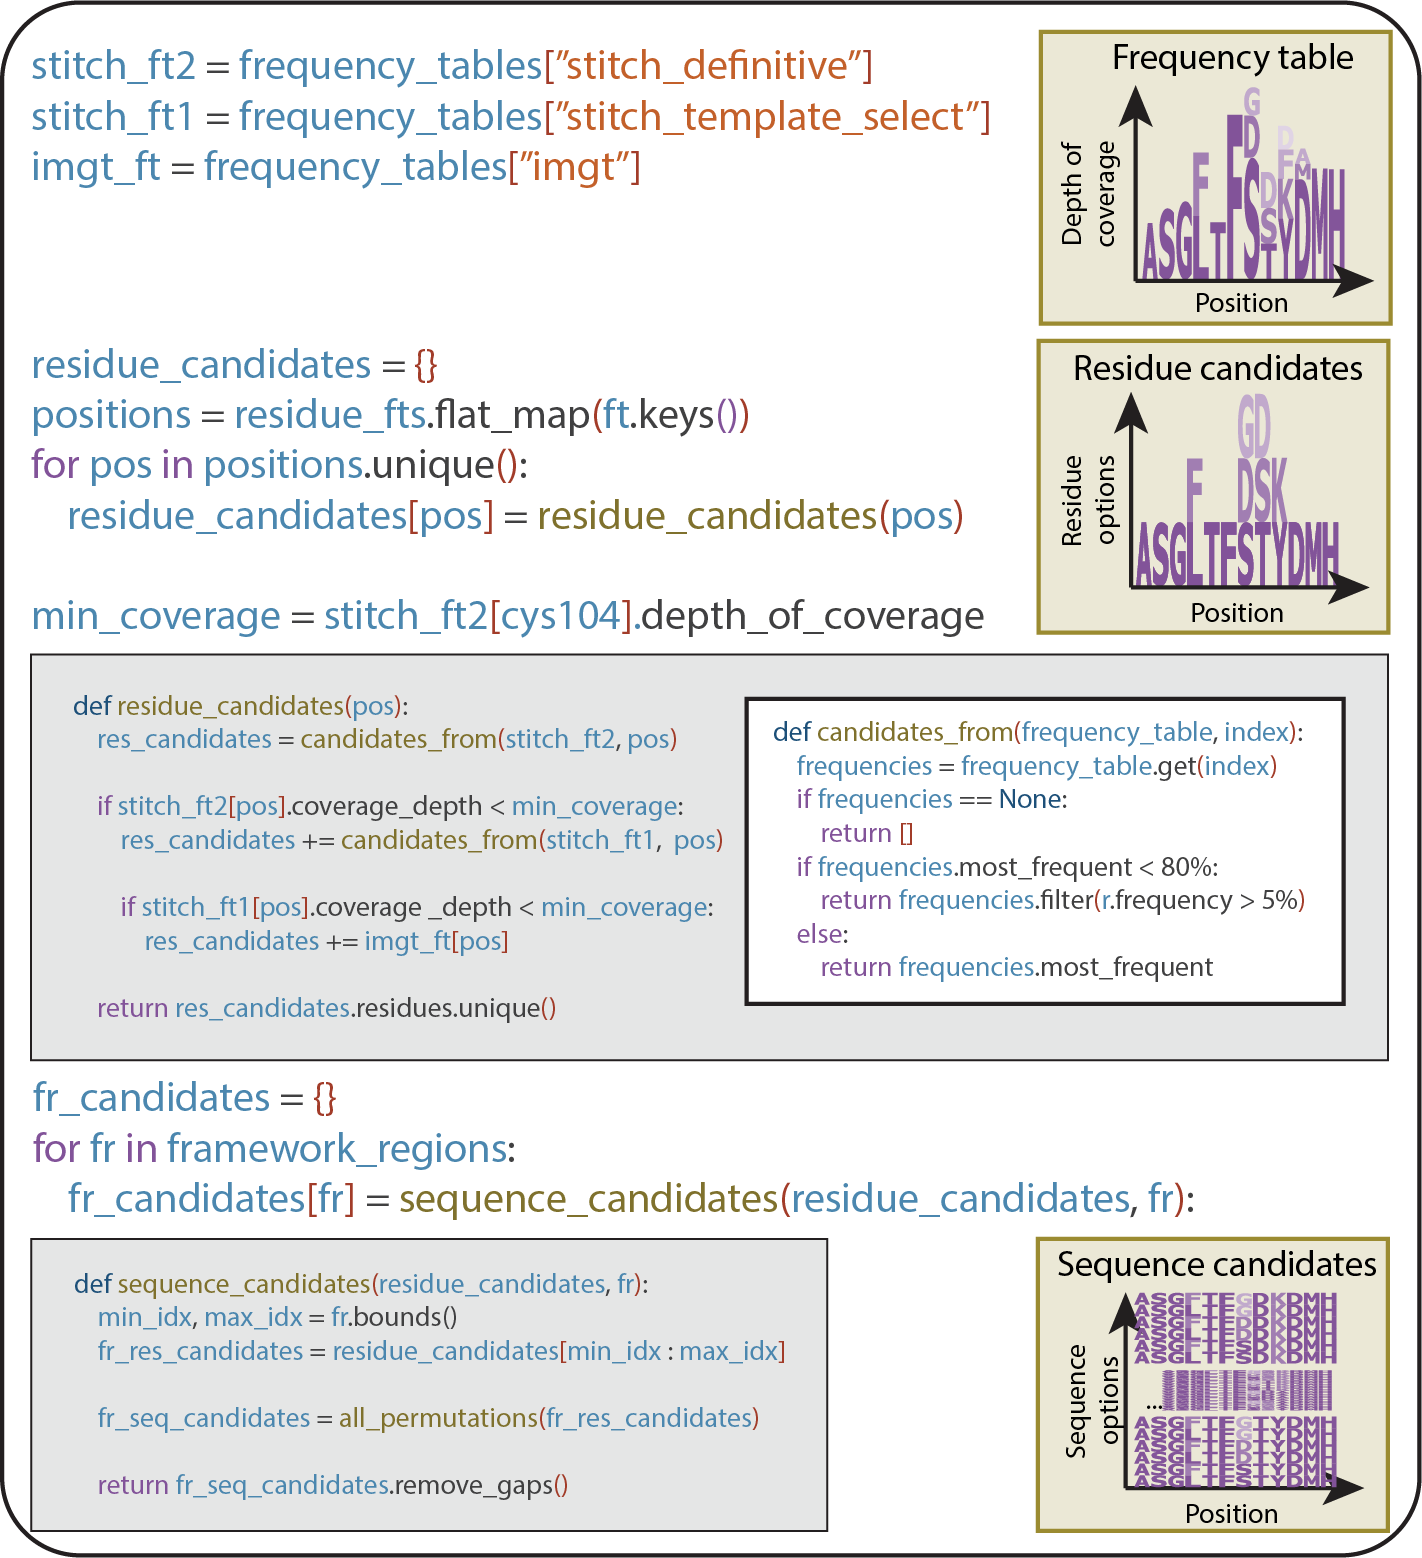
\includegraphics[]{Chapter.5/Figures/fs1.png}
    \caption{\textbf{Framework region candidate generation.} Candidate FR sequences for each framework region are generated from residue frequency tables from three sources: The definitive Stitch run, the template selection Stitch run and the IMGT (from highest to lowest priority respectively). Residue candidates are selected based on their relative frequency. For each position, residue candidates from the next frequency table are only taken if the depth of coverage in the current table is lower than the depth of coverage at the highly conserved Cys104. After residue candidates have been selected for all positions, all permutations of these candidates are taken for each FR to yield sequence candidates for these FRs.}
    \label{fig:figs5.1}
  \end{figure*}
  \begin{figure*}[!htb]
    \center
    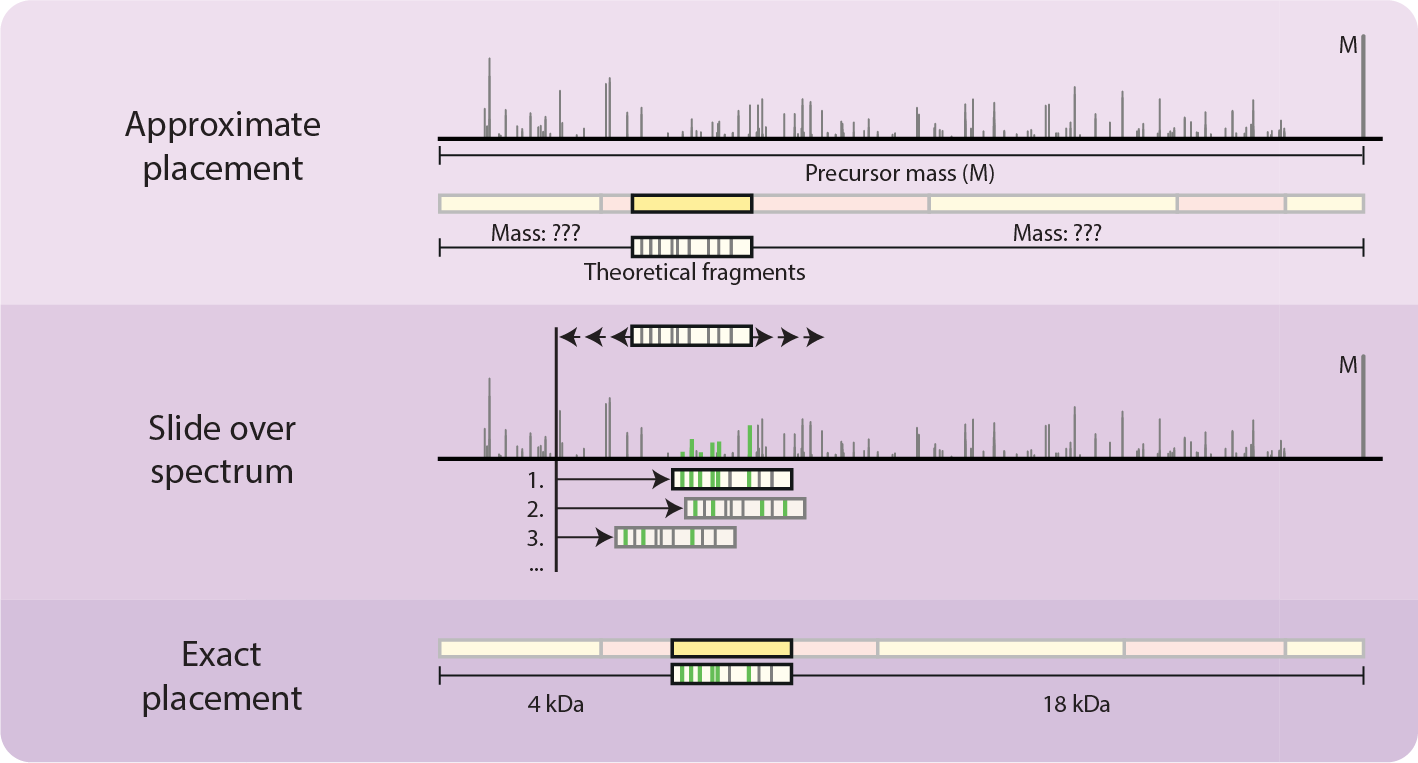
\includegraphics[]{Chapter.5/Figures/fs2.png}
    \caption{\textbf{Schematic of the sliding window fragment matching algorithm.} The sliding window fragment matching algorithm finds the optimum mass offset for an imperfect subsequence for a given fragmentation spectrum (FR2 in the figure). Theoretical fragments are generated at an approximate offset and shifted by a predefined increment (default: 0.01 Da) throughout a predefined range (default: starting position plus and minus 190 Da). This enables error-tolerant scoring of subsequences and determination of the prefix- and suffix- (N- and C-terminal) masses.
    }
    \label{fig:figs5.2}
  \end{figure*}


  \begin{table*}[!hbt]
    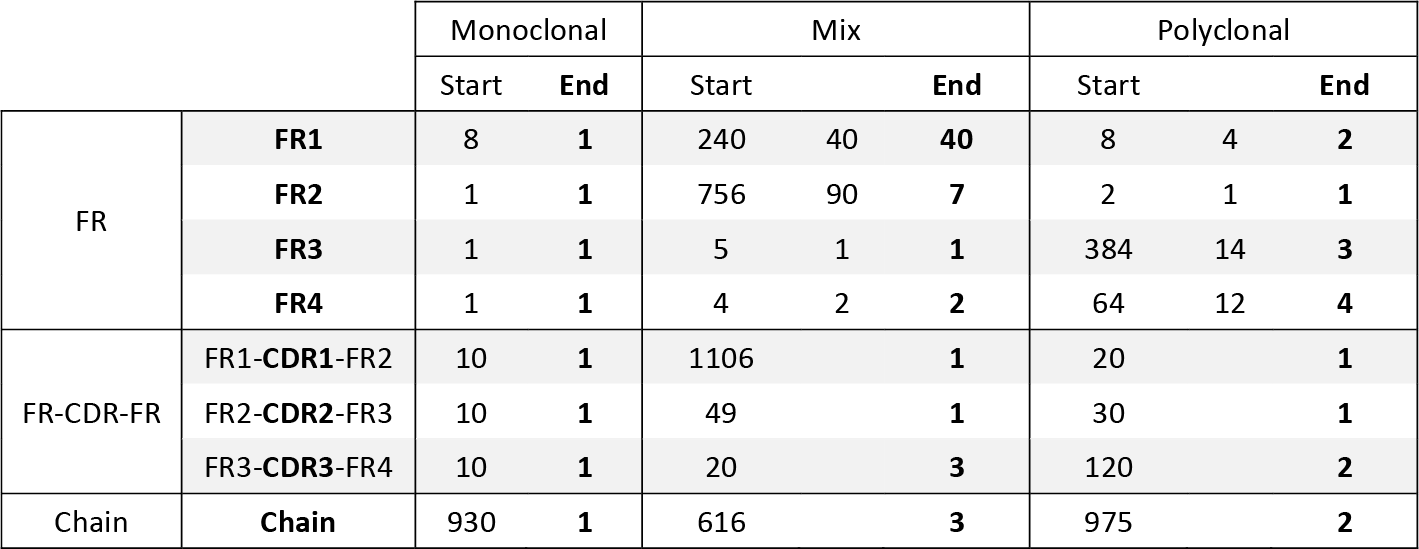
\includegraphics[]{Chapter.5/Figures/ts2.png}
    \caption{
      \textbf{Number of segment candidates throughout the workflow.} The table shows the number of segment candidates at the start and end of each stage. For the mix and polyclonal FR sequencing stage, a middle column is included which displays the number of candidates after a “first pass” filtering, for example excluding candidates that do not have highly conserved residues (Cys23 and Cys104 specifically), or candidates with highly unlikely terminal mass offsets.
    }
    \label{tab:tabs5.2}
  \end{table*}

  \begin{figure*}[!pt]
    \center
    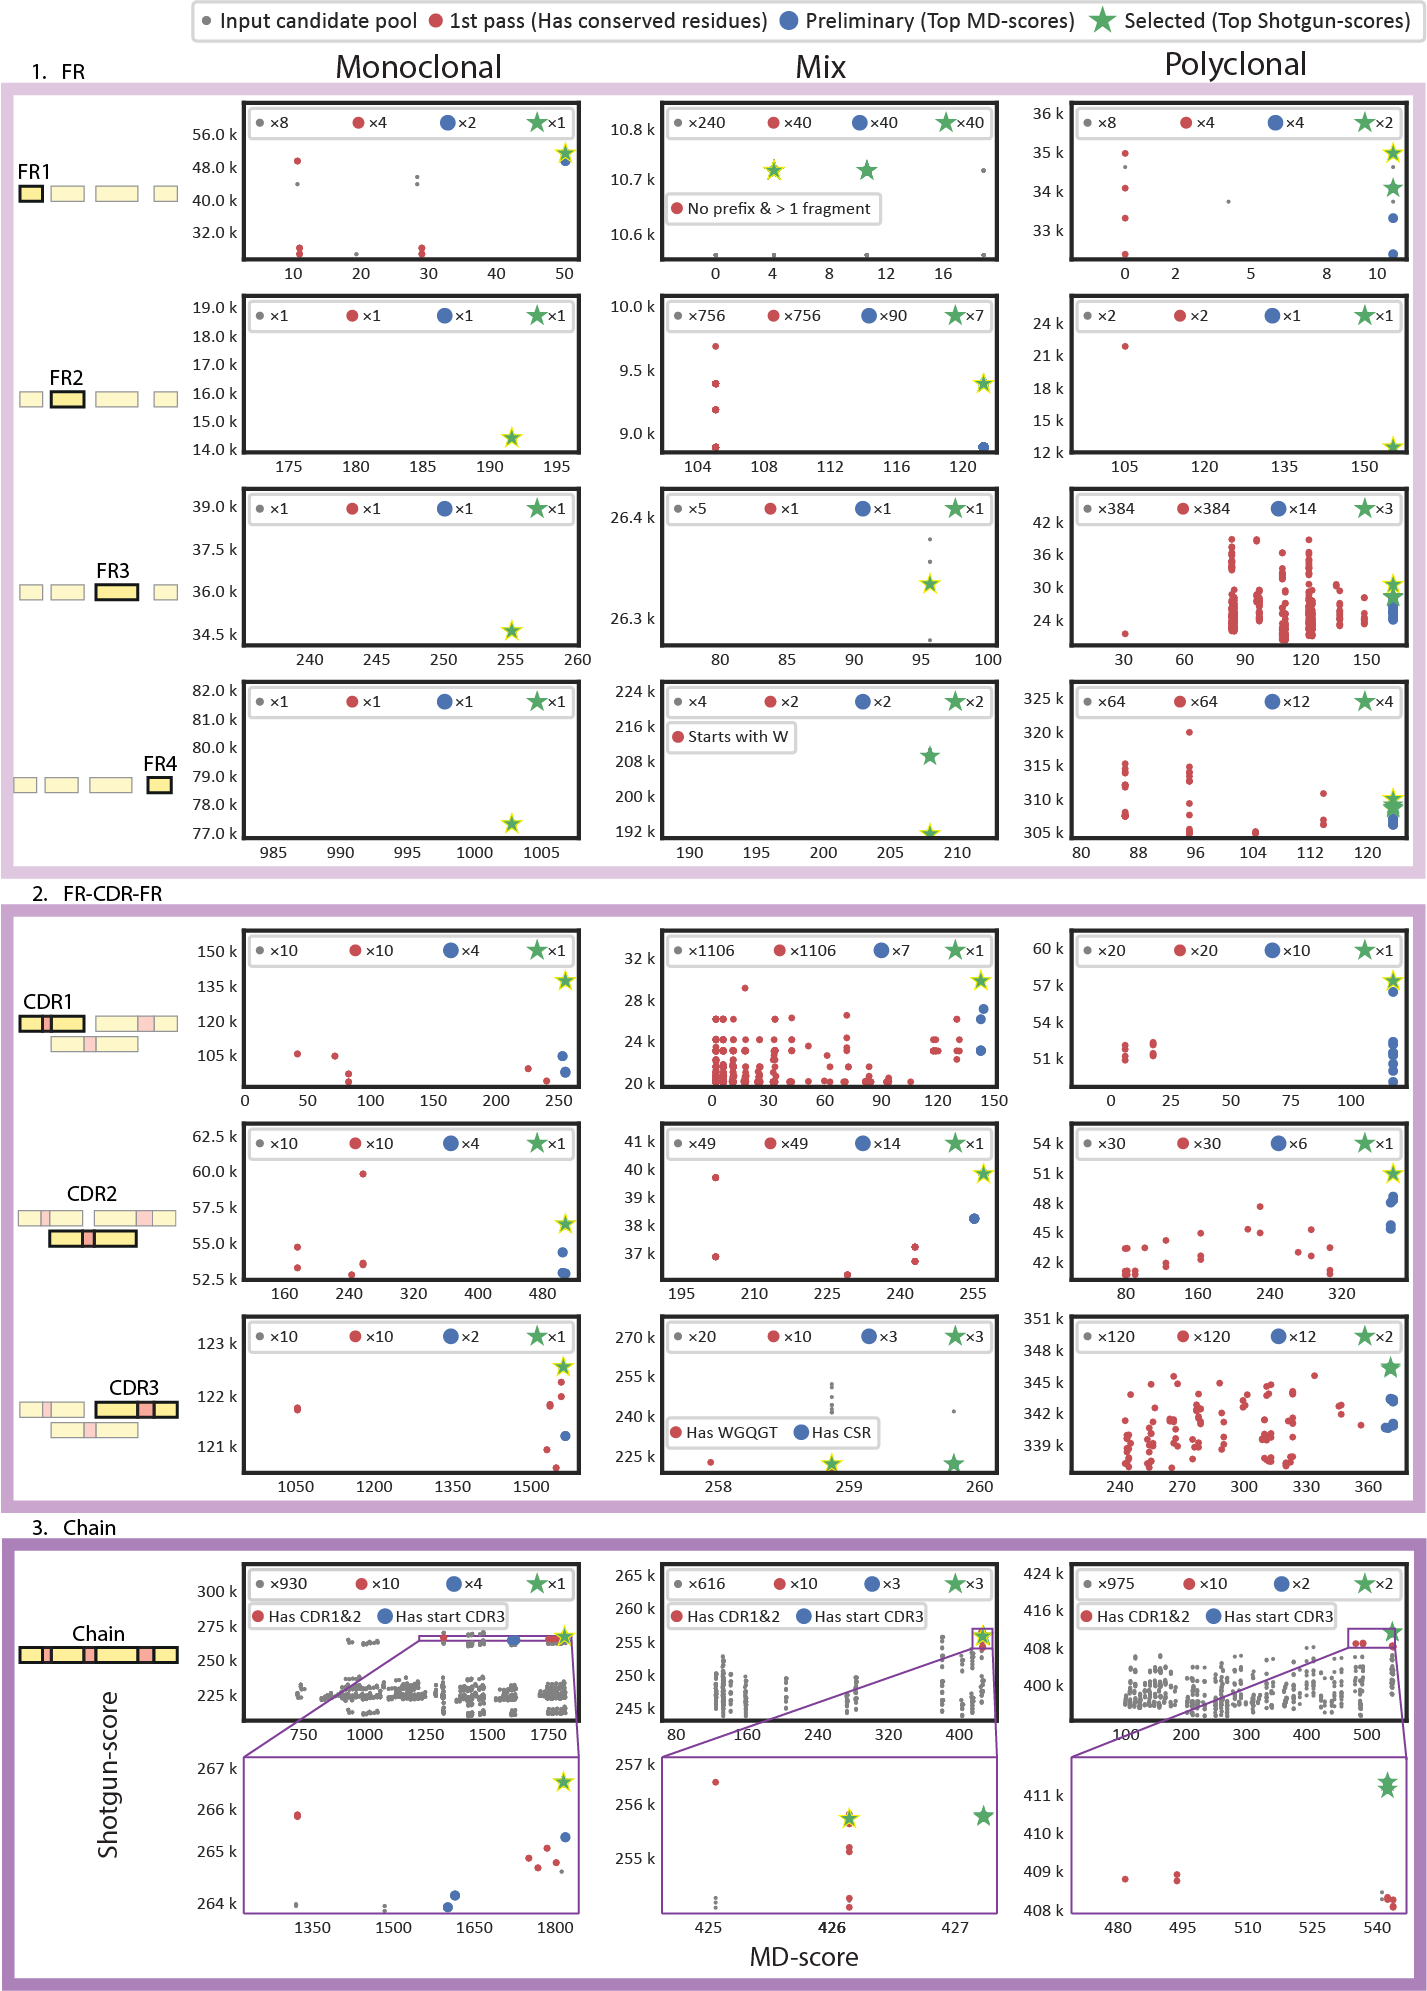
\includegraphics[]{Chapter.5/Figures/fs3.png}
    \captionsetup{singlelinecheck = false, format= hang}
    \caption{
      Figure legend on next page.
    }
    \label{fig:figs5.3}
  \end{figure*}
  \addtocounter{figure}{-1}
  \begin{figure*}[!ht]
    \caption{\textbf{BU- and MD- based scoring and germline-based selection criteria enable effective segment candidate selection throughout the workflow.} Score distributions (MD-score (x axis) and Shotgun-score (y axis)) for all considered segment candidates are shown. Each column depicts segment candidates for a sample. Each graph represents segment candidate scores for a target segment. Each dot in the graphs represents a rejected candidate, whereas stars indicate selected candidates. A yellow outline highlights the correct candidate. The correct candidate was selected in all stages (except for the CDR3 and chain for the polyclonal sample, where it was not present.) However, ambiguity could not be fully resolved everywhere. A legend with the consecutive selection criteria is shown at the top of the figure. Grey: Input candidate. Red: First pass criteria met (default criterium: Has conserved Cys23 or Cys104). Blue: Preliminary selection criterium met (default criterium: MD-score was <5 removed from the maximum in the pool). Green: Selected for the next stage (default criterium: Top Shotgun-score). Any additional/alternative criteria are shown in the graph itself (e.g., for the mix FR4 candidate pool, the first pass filtering criterium included the presence of Trp118). The number of candidates satisfying each criterium is given at the top of each graph. E.g., for the monoclonal, 8 FR1 candidates were considered in total. Of these 8, only 4 had the highly conserved Cys23. Of these 4, only 2 were considered top candidates based on their MD-score. A single candidate was finally selected for the next stage.}
    \vspace{24cm}
  \end{figure*}



  \begin{table*}[!hbt]
    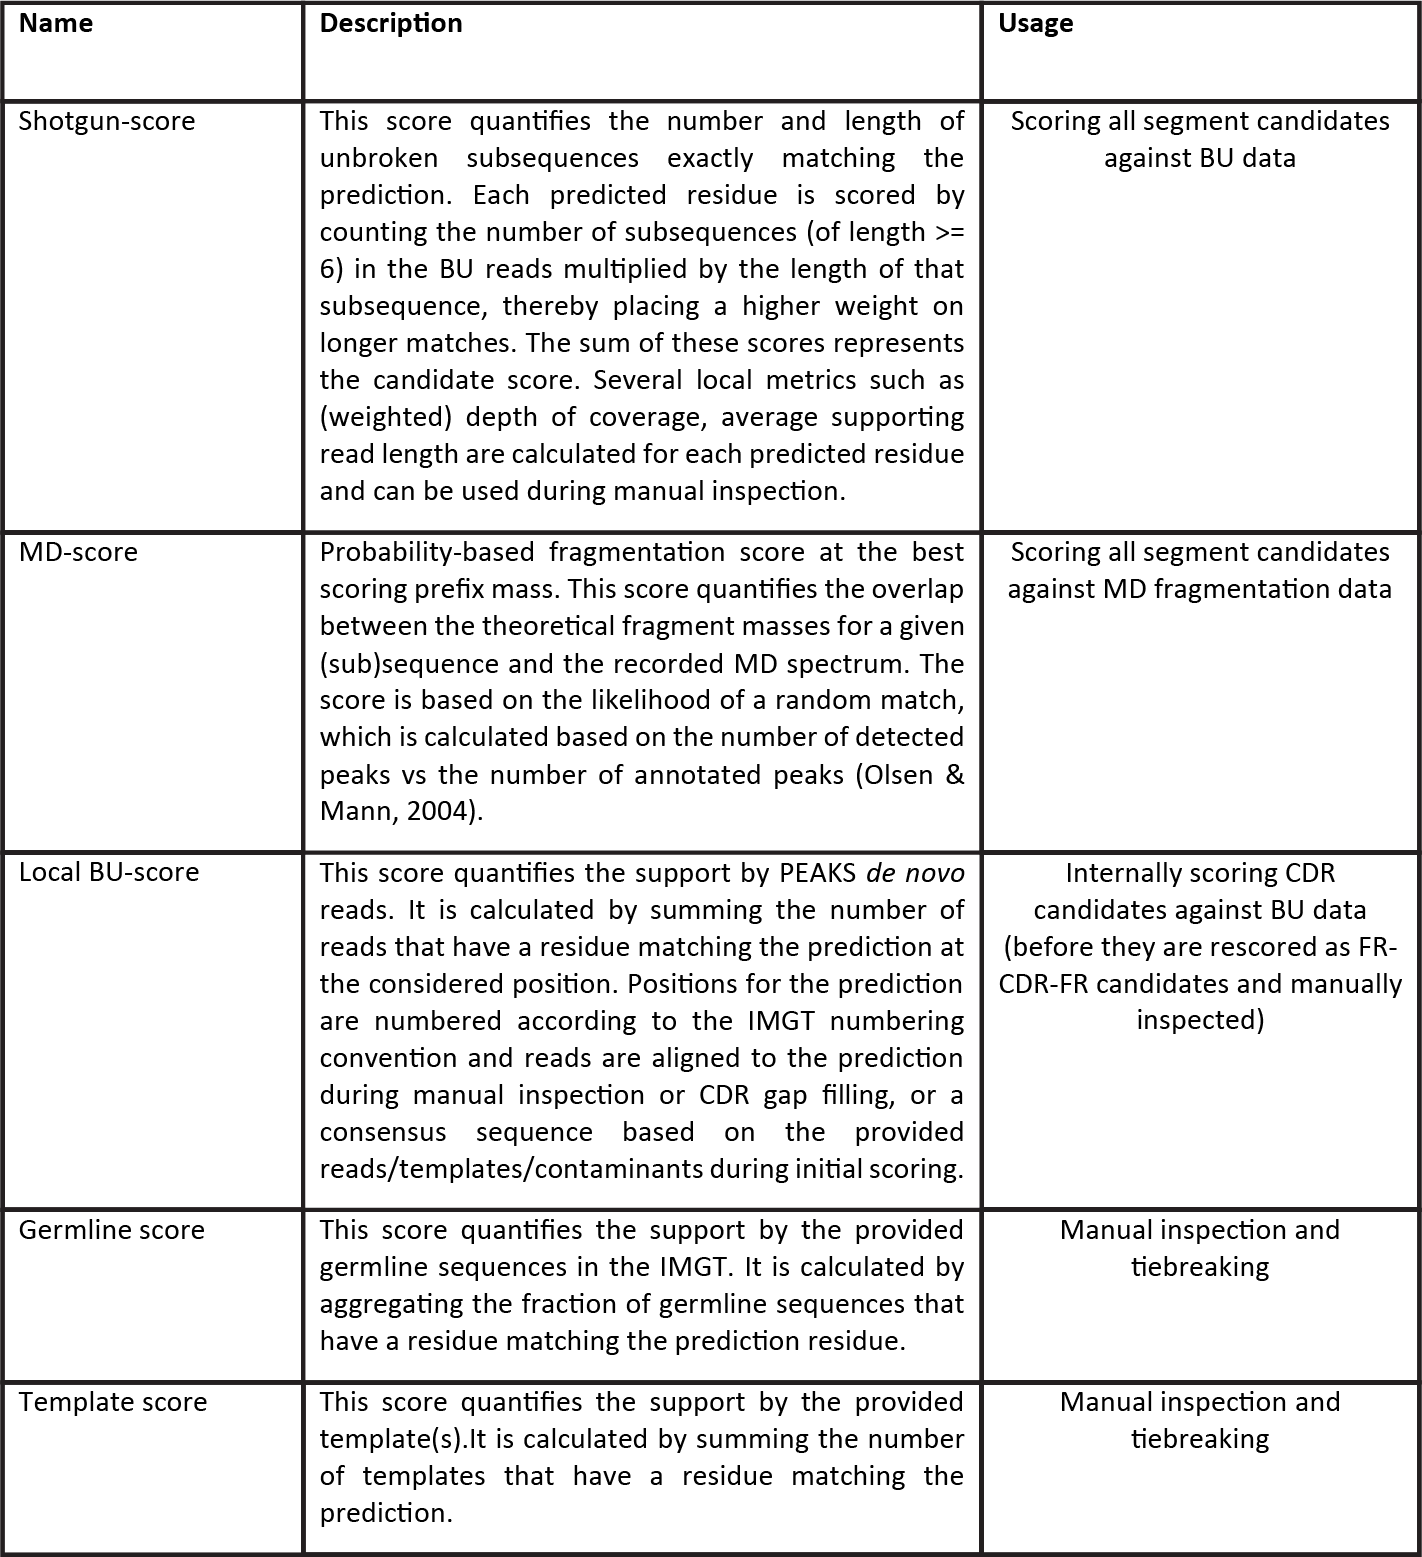
\includegraphics[]{Chapter.5/Figures/ts3.png}
    \caption{
      \textbf{Different scores calculated throughout the workflow.} The Template- and Germline- score are not used in the manuscript. The local BU-score is only used for internal ranking before CDR rescoring as the CDR-candidate are too short for the Shotgun-score.
    }
    \label{tab:tabs5.3}
  \end{table*}


  \begin{figure*}[!htb]
    \center
    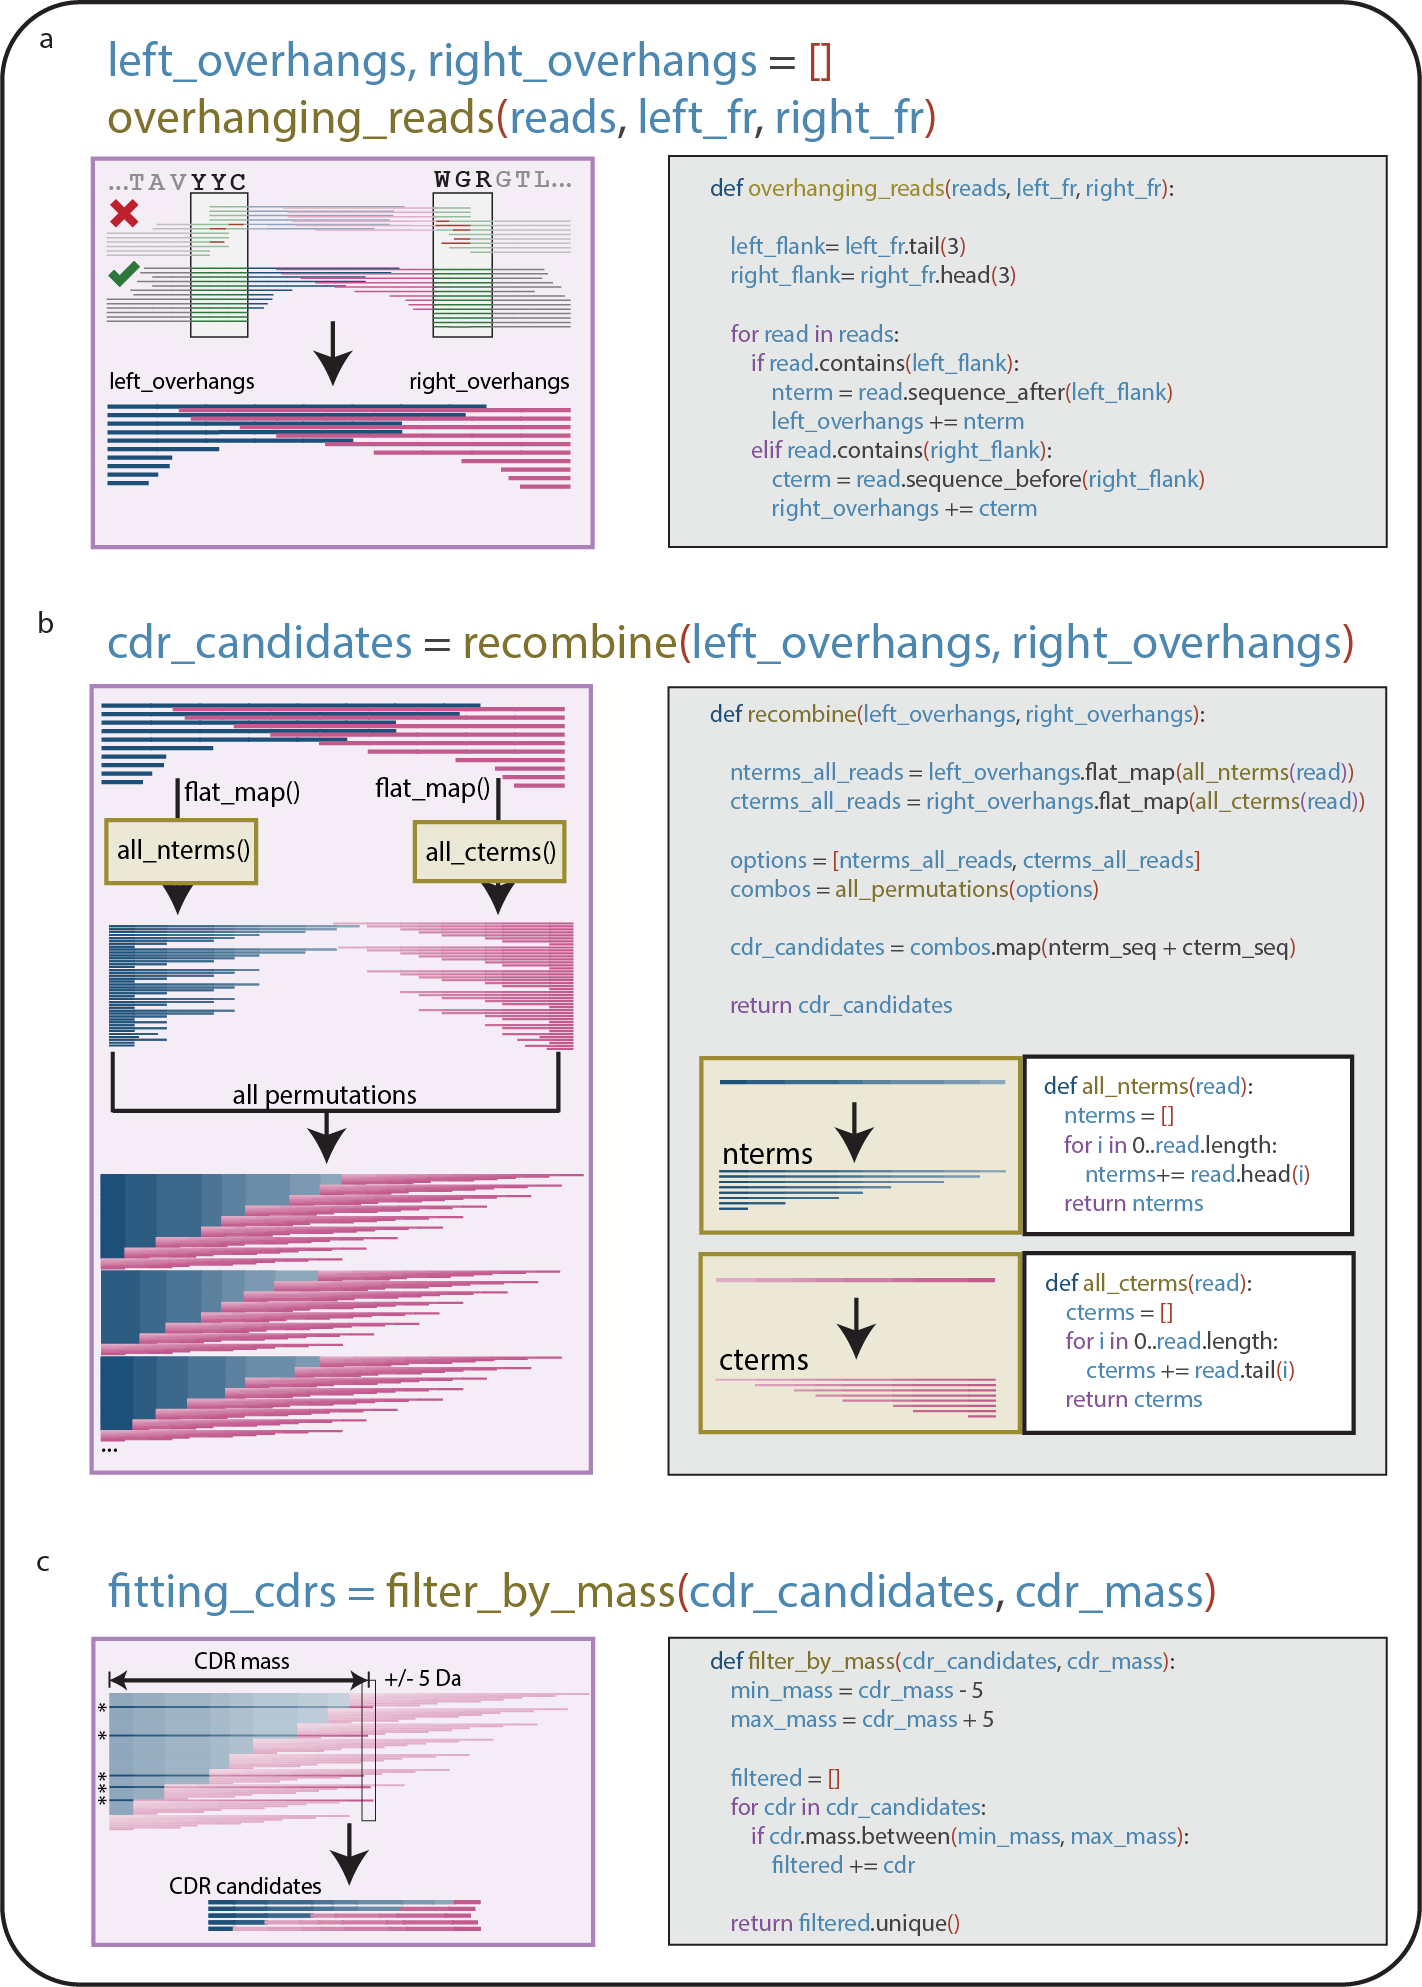
\includegraphics[]{Chapter.5/Figures/fs4.png}
    \caption{\textbf{CDR candidate generation.} Candidate CDR sequences are generated by joining a pair of adjacent FR candidates (e.g. a FR1 candidate and a FR2 candidate) using overhanging reads from both FRs. ~~a) Reads containing the 3 CDR flanking residues are taken for the left (e.g. FR1) and right FR (e.g. FR2). ~~b) The N-terminal overhanging reads (left\_overhangs) are then combined with the C-terminal overhanging reads (right\_overhangs), generating all possible combinations. ~~c) The mass of the CDR is calculated using the FR candidates and the \emph{sliding window score} (\textbf{\autoref{fig:figs5.2}}) and used to filter the CDR candidates, retaining only those matching the target mass within a 5 Da tolerance.}
    \label{fig:figs5.4}
  \end{figure*}

\end{subappendices}


\clearpage
\section*{References}
\bibliographystyle{Stylesettings/pnas}
\patchcmd{\thebibliography}
{\clubpenalty 4000\widowpenalty 4000}
{\clubpenalties 1 10000 \widowpenalties 1 10000}
{}{}
\bibliography{chapmerge}
\stopthumb


